\documentclass[titlepage,12pt]{article}


\usepackage[utf8]{inputenc}
\usepackage[spanish]{babel}
\usepackage{cancel}
\usepackage{graphicx}
\usepackage{subcaption}
\usepackage{caption}
\usepackage{float} % colocar donde quieras las figuras con [H]
\usepackage{lipsum}
\usepackage{mathtools}
\usepackage{amsmath}
\usepackage{amssymb}
\usepackage{xcolor}
\usepackage[colorlinks=true,urlcolor=blue,linkcolor=black,citecolor=red]{hyperref}
\usepackage[a4paper,margin=2cm]{geometry}


\numberwithin{equation}{section}
\setlength{\parindent}{0.8cm}

\title{\textbf{Almacenamiento de memoria y transiciones de fase en una red de Hopfield}}
\author{Julián López Carballal, Jorge García Beni, Rubén de San Juan Morales, Fernando García Sánchez y José Luis Miranda Mora}
\date{\today}

\begin{document}
	\maketitle
	\fontsize{15pt}{0}\tableofcontents
	\newpage
	
	
	\section{Red de Hopfield}
	\fontsize{12pt}{0}
	La red de Hopfield es un modelo de red neuronal propuesto por Hopfield en 1982 \cite{hopfield82}. Se trata de una red formada por $N$ neuronas, las cuales sólo pueden tener dos estados: $\sigma_i = +1$ (``encendido'') o $\sigma_i=-1$ (``apagado''), los cuales evolucionan en el tiempo, de forma discreta con pasos temporales finitos $\Delta t$. Estas neuronas interaccionarán entre sí con pesos $J_{ij}$, de modo que el potencial sobre una de las neuronas debido a su interacción con las demás es:
	\begin{displaymath}
	\Phi_i(t)=\sum_{j\neq i} J_{ij}\sigma_j
	\end{displaymath}
	El fin de estas redes es el almacenamiento y la reproducción de patrones. Podemos definir un patrón $\mu$ como una configuración dada de la red, $\mathcal{P}^\mu_i = \pm1, i \in[1,N]$. Entonces, considerando que la evolución de los estados neuronales se da en pasos temporales finitos $\Delta t$, la red habrá reproducido correctamente el patrón $\mu$ si $\sigma_i(t)=\sigma_i(t+\Delta t)=\mathcal{P}^\mu_i$; o dicho de otro modo, los patrones deberán ser puntos fijos de la dinámica. En general, consideraremos que la red almacena un número $K$ de patrones, de modo que $\mu\in[1,K]$. También consideraremos que los patrones sean ortogonales, de modo que:
	\begin{equation} \label{ortogonal}
	\frac{1}{N}\sum_{i=1}^N \mathcal{P}^\mu_i \mathcal{P}^\nu_i = \delta^{\mu\nu}
	\label{ortpat}
	\end{equation}
	\subsection{Analogía con sistemas magnéticos. Hamiltoniano de Ising}
	Este modelo es muy similar al modelo de Ising para un sistema magnético. Acogiéndonos a esta analogía, bajo la restricción de simetría en las interacciones ($J_{ij}=J_{ji}$), podemos utilizar el hamiltoniano del modelo de Ising (a campo magnético $\vec{B}=0$, situación para la que se puede observar la transición ferromagnético-paramagnético) para la dinámica de un sistema de espines $\sigma_i$ a una temperatura $T$, para describir la dinámica de nuestra red de Hopfield.
	\begin{equation}
	H = \frac{1}{2}\sum_{i}\sum_{j\neq i}J_{ij}\sigma_i\sigma_j
	\label{HIsing}
	\end{equation}
	dada la utilidad de esta analogía, por comodidad y abusando del lenguaje, llamaremos ``espines'' a los estados de las neuronas $\sigma_i$ que hemos definido anteriormente. 

	Podemos cuantificar la similitud entre el estado en el que se encuentra la red $\sigma_i$ y el patrón que buscamos reproducir $\mathcal{P}^\mu_i$ definiendo el solapamiento:
	\begin{equation}
	m^\mu(t)=\frac{1}{N}\sum_i \mathcal{P}^\mu_i\sigma_i(t)
	\label{overlap}
	\end{equation}
	que toma el valor máximo $m^\mu = 1$ cuando la red reproduce exactamente el patrón, es decir, $\sigma_i = \mathcal{P}^\mu_i\hspace{0.2cm}\forall i$.
	
	Estos estados estacionarios vienen determinados por la forma de los pesos de la interacción $J_{ij}$, es decir, son los responsables del almacenamiento de los patrones $\mathcal{P}^\mu_i$. Recordemos que hemos elegido el caso simétrico, $J_{ij}=J_{ji}$. Estos pesos pueden interpretarse como elementos de una matriz. Si queremos que nuestra red sea capaz de reproducir (recordar) un número $K$ de patrones $\mathcal{P}^\mu_i$ previamente almacenados, buscamos que los $J_{ij}$ establezcan una correlación entre los estados y el patrón. Para ello, la forma más simple que pueden tomar es:
	\begin{equation} \label{J-eq}
	J_{ij}=\frac{1}{N}\sum_{\mu=1}^K \mathcal{P}^\mu_i \mathcal{P}^\mu_j
	\label{Jint}
	\end{equation}
	dónde $N$ es el número de neuronas (o espines) en la red; en el límite termodinámico (LT), $N\rightarrow\infty$ mientras que para una red finita $D$-dimensional de lado $L$, $N=L^D$. Recordemos que $\mathcal{P}^\mu_i = \pm1$, y que los patrones ortogonales de modo que los $\mathcal{P}^\mu_i$ satisfacen \eqref{ortpat}.
	\section{Generalización del modelo de Hopfield}
	Hasta ahora hemos visto que la red de Hopfield admite ser interpretada como un modelo de Ising, por su analogía con un sistema magnético de espines que sólo pueden tener dos orientaciones posibles. Además, la red de Hopfield sigue una dinámica dónde, empezando desde una configuración arbitraria, el sistema evoluciona a través de una secuencia de cambios de espín (que involucra aquellos espines desalineados con sus campos moleculares). En esencia, esta es una dinámica de Monte Carlo o Glauber, dónde el proceso produce un decrecimiento monótono del hamiltoniano \eqref{HIsing}, es decir, disminuye la energía. Sin embargo, hasta ahora hemos tratado un sistema sin ruido; en un sistema con ruido se pueden llegar a configuraciones fuera de la dinámica que estamos tratando. Para solventar este problema, se introduce una temperatura efectiva $T$ que caracteriza el nivel de ruido en el sistema \cite{amit1}. La generalización natural del modelo a un sistema con dicho ruido es adoptar la dinámica de espines de Glauber a una temperatura finita $T$, dónde la distribución de las configuraciones se relaja a una distribución de Gibbs.
	\begin{displaymath}
	P(\lbrace\sigma\rbrace)\propto e^{-H(\lbrace\sigma\rbrace)/T}
	\end{displaymath}
	Este modelo se conoce como el modelo de Hopfield generalizado. En este nuevo caso, la estabilidad de un estado a todos los cambios de espín individuales no es suficiente para la estabilidad dinámica a temperaturas finitas. 
	\subsection{Teoría de campo medio para el modelo}
	Ahora, estudiemos el hamiltoniano \eqref{HIsing} con los pesos de interacción \eqref{Jint}, para un número de patrones o memorias $K$ finito. Posteriormente tomaremos el LT, $N\rightarrow\infty$. La densidad de energía libre será:
	\begin{equation}
	f(T)=-\frac{T}{N}\left<\log Z\right>_{\mathcal{P}}
	\label{famit}
	\end{equation}
	dónde $\left<\cdot\right>_\mathcal{P}$ es el promedio sobre la distribución de patrones $\lbrace\mathcal{P}^\mu_i\rbrace$ y $Z$ es la función de partición.
	\begin{equation}
	Z=\sum_{\lbrace\sigma\rbrace}e^{-H(\lbrace\sigma\rbrace)/T}=\left(\frac{N}{T}\right)^{\frac{K}{2}}e^{-\frac{K}{2T}}\int\prod_\mu \frac{dm^\mu}{\sqrt{2\pi}}\exp\Bigg\{-\frac{N\vec{m}^2}{2T}+\sum_i \log\left[2\cosh\left(\frac{\vec{m}\cdot\vec{\mathcal{P}_i}}{T}\right)\right]\Bigg\}
	\label{Zamit}
	\end{equation}
	dónde hemos introducido la cantidad $m^\mu$, y la notación vectorial $\vec{m}$ y $\vec{\mathcal{P}_i}$, cuyas componentes son los $K$ valores de ambas cantidades. $\vec{m}$ será el parámetro de orden. Si $K$ es finito, la integral estará predominada por su valor de punto de silla, con lo que tenemos:
	\begin{equation}
	-\frac{T\ln Z}{N}=\frac{1}{2}\vec{m}^2-\frac{T}{N}\sum_i\ln\left[2\cosh\left(\frac{\vec{m}\cdot\vec{\mathcal{P}_i}}{T}\right)\right]
	\label{saddlepoint}
	\end{equation}
	y el parámetro de orden viene dado por la ecuación $\partial\ln Z/\partial m^\mu$=0.
	\begin{equation}
	\vec{m}=\frac{1}{N}\sum_i \vec{\mathcal{P}_i}\tanh\left(\frac{\vec{m}\cdot\vec{\mathcal{P}_i}}{T}\right)
	\label{eqm}
	\end{equation}
	para $N$ finito el lado derecho de estas ecuaciones depende de la distribución concreta de patrones, pero en el LT las fluctuaciones se suprimen y las cantidades $\ln Z$ y $\vec{m}$ están auto-promediadas; por tanto, las sumas $(1/N)\sum_i$ se convierten en promedios sobre la distribución {$\vec{\mathcal{P}_i}$}, de dónde obtenemos las ecuaciones de campo medio:
	\begin{equation}
	f(T)=\frac{1}{2}\vec{m}^2 - T\left<\log\left[2\cosh\left(\frac{\vec{m}\cdot\vec{\mathcal{P}_i}}{T}\right)\right]\right>_{\mathcal{P}}
	\label{meanfieldf}
	\end{equation}
	\begin{equation}
	\vec{m}=\left<\vec{\mathcal{P}_i}\cdot\tanh\left(\frac{\vec{m}\cdot\vec{\mathcal{P}_i}}{T}\right)\right>_{\mathcal{P}}
	\label{meanfieldm}
	\end{equation}
	si ahora introducimos el promedio térmico de los espines:
	\begin{equation}
	\left<\sigma_i\right>=\tanh\left(\frac{\vec{m}\cdot\vec{\mathcal{P}_i}}{T}\right)
	\label{thermalspin}
	\end{equation}
	introduciendo \eqref{thermalspin} en \eqref{meanfieldm} obtenemos:
	\begin{equation}
	m^\mu=\left<\mathcal{P}^\mu_i{\left<\sigma_i\right>}\right>_{\mathcal{P}}
	\label{meanfieldoverlap}
	\end{equation}
	comparando \eqref{meanfieldoverlap} con \eqref{overlap}, vemos que el parámetro de orden $\vec{m}$ es el solapamiento promedio. De hecho, esta comparación es más fácil con la ecuación \eqref{meanfieldm}, antes de eliminar el sumatorio que también aparece en \eqref{overlap}. Aquí podemos ver una analogía con el modelo de Ising. En él, el parámetro de orden --la magnetización-- para campo medio tiene la siguiente forma:
	\begin{displaymath}
	\tilde{m}=\left<\sigma_i\right>
	\end{displaymath}
	que es similar a la forma que ha tomado nuestro parámetro de orden, el solapamiento, en \eqref{meanfieldoverlap}. Veremos que esta analogía se puede extender más en el siguiente apartado.
	\subsection{Distribución de los patrones. Estados de Mattis}
	Estudiemos ahora la distribución de los estados que conforman los patrones. Cómo ya hemos establecido en la sección 1, un espín $i$ que forma parte del patrón $\mu$ sólo puede tomar dos valores: $\mathcal{P}^\mu_i=+1$ o $\mathcal{P}^\mu_i=-1$. Entonces, sabemos inmediatamente que hay un 50\% de probabilidad de que $\mathcal{P}^\mu_i$ se encuentre en el primer caso, y otro 50\% de que se encuentre en el segundo. Esto nos da directamente la distribución para un único espín del patrón, que matemáticamente podemos escribir cómo:
	\begin{equation}
	p(\mathcal{P}^\mu_i)=\frac{1}{2}\left[\delta(\mathcal{P}^\mu_i + 1) + \delta(\mathcal{P}^\mu_i - 1)\right]
	\label{distpatind}
	\end{equation}
	Con este resultado en mano, podemos escribir la distribución para los K patrones (o lo que es lo mismo, para $\vec{\mathcal{P}_i}$) cómo:
	\begin{equation}
	P(\lbrace\mathcal{P}^\mu_i\rbrace)=\prod_{\mu,i}p(\mathcal{P}^\mu_i)
	\label{distpat}
	\end{equation}
	Ahora, el desarrollo en serie de potencias de $\vec{m}$ de las ecuaciones \eqref{meanfieldf} y \eqref{meanfieldm} es:
	\begin{align}
	f=&-T\log 2 + \frac{1}{2}(1 - \beta)\vec{m}^2 + o(\vec{m}^4) \label{fseries}\\ m^\mu=&\beta m^\mu + \frac{2}{3}\beta^3 (m^\mu)^3 - \beta^3m^\mu\vec{m}^2 + o(\vec{m}^4) \label{mseries}
	\end{align}
	con $\beta\equiv1/T$ (trabajamos en unidades $k_B=1$). Vemos en \eqref{fseries} que para $T=1$, $f=-T\log2$; y despreciando en el término cúbico en $m^\mu$ a la derecha podemos escribir una versión aproximada de \eqref{mseries}:
	\begin{displaymath}
	m^\mu\approx(\beta-\beta^3\vec{m}^2)m^\mu
	\end{displaymath}
	Si evaluamos esta aproximación en $T=1$, o lo que es igual, $\beta=1$, tenemos que la única solución posible es $\vec{m}=0$ (estado ``paramagnético''), que implica de nuevo por la ecuación \eqref{fseries} $f=-T\log2$. Para $T>1$, $\beta<1$, por lo que la aproximación que hemos tomado en \eqref{mseries} tiene mayor validez y por tanto podemos concluir que la única solución sigue siendo $\vec{m}=0$, y $f=-T\log 2$. Alternativamente, podemos argumentar que sí $T >> 1$, $\beta << 1$ y directamente por \eqref{mseries} $m^\mu \approx 0\,\,\forall\mu$, lo que implica $\vec{m}=0$. 
	
	Esta solución se vuelve inestable sin embargo, por debajo de la temperatura crítica $T_c=1$, dónde aparecerán soluciones con $m^\mu$ no nulas. Por ello definiremos la dimensionalidad de $\vec{m}$, $n$: el número de componentes no nulas de $\vec{m}$ para una solución con $T<1$. Estamos ahora observando un comportamiento crítico; sin embargo, esto no debe sorprendernos pues el modelo que estamos utilizando un modelo inspirado en el modelo de Ising, cuyo fin original es describir sistemas magnéticos donde efectivamente hay un comportamiento crítico, la transición ferromagnético-paramagnético. Se puede ver en \eqref{meanfieldm} y \eqref{distpatind} que alterar el orden o cambiar el signo de las $n$ componentes no nulas no altera las soluciones.
	
	Veamos ahora el caso $n=1$. Este caso es especialmente interesante porque nos devolverá las ecuaciones del modelo de Ising para sistemas magnéticos en campo medio. Supongamos $m^1=m\neq0$ y $m^\mu = 0\,\,\forall \mu>1$. Entonces:
	\begin{equation}
	f=\frac{1}{2}m^2 - T\log\left[2\cosh(\beta m)\right]
	\label{fIsinglike}
	\end{equation}
	\begin{equation}
	m=\tanh(\beta m)
	\label{mIsinglike}
	\end{equation}
	Estas soluciones corresponden a un estado dónde:
	\begin{equation}
	\left<\sigma_i\right>=\mathcal{P}_i^1\tanh(\beta m)
	\label{mattisstate}
	\end{equation}
	si introducimos esta solución en \eqref{meanfieldoverlap} tenemos $m=\left<(\mathcal{P}_i^1)^2\tanh(\beta m)\right>_{\mathcal{P}}$. Cómo $\mathcal{P}^\mu_i=\pm 1$, esto se convierte en $m=\left<\tanh(\beta m)\right>_{\mathcal{P}}$ y, por último, al no aparecer los estados de los patrones, el promedio desaparece. Hemos recuperado \eqref{mIsinglike}. 
	
	El estado \eqref{mattisstate} es equivalente termodinámicamente al estado ferromagnético del modelo de Ising. Existen $2K$ estados de este tipo correspondientes a distintas $\mu$ y a distintos signos de las componentes $m^\mu$. Estos estados se denominan estados de Mattis.
	\\
	
	Los estados de Mattis son mínimos globales de la energía libre para $T=0$. Podemos probar esto para el estado anterior \eqref{mattisstate}, que correspondía al caso $n=1$. Dado que en $T=0$, $\beta=\infty$, para evaluar \eqref{mIsinglike} en $T=0$ necesitamos el siguiente límite, teniendo en cuenta que $m>0$.
	\begin{equation}
	\lim_{x\rightarrow\infty}\tanh mx =\lim_{x\rightarrow\infty} \frac{e^{mx} - \cancel{e^{-mx}}}{e^{mx} + \cancel{e^{-mx}}}=\lim_{x\rightarrow\infty} \frac{e^{mx}}{e^{mx}}=1
	\label{lim1}
	\end{equation}
	De modo que:
	\begin{equation}
	m_{(n=1)}(T=0)=\lim_{\beta\rightarrow\infty}\tanh(\beta m)=1
	\label{mMattisT0}
	\end{equation}
	Para evaluar ahora la energía libre necesitamos el siguiente límite:
	\begin{equation}
	\lim_{x\rightarrow\infty}\frac{1}{x}\log\left(2\cosh mx\right)=\lim_{x\rightarrow\infty}\frac{1}{x}\log\left(e^{mx} + e^{-mx}\right)=\lim_{x\rightarrow\infty}\frac{1}{x}\log\left(e^{mx} + \cancel{e^{-mx}}\right)=1
	\label{lim2}
	\end{equation}
	Tomando ahora el resultado \eqref{mMattisT0} e introduciéndolo en \eqref{fIsinglike}, junto con el límite \eqref{lim2}:
	\begin{equation}
	f_{(n=1)}(T=0)=\frac{1}{2}-\lim_{T\rightarrow0}T\log\left[2\cosh(\beta m)\right]=\frac{1}{2} - 0\cdot1=\frac{1}{2}
	\label{fMattisT0}
	\end{equation}
	
	Veamos ahora que efectivamente \eqref{fMattisT0} es el valor mínimo que puede tomar la energía libre. Para ello tendremos que tomar el límite $T\rightarrow0$ en las ecuaciones de campo medio, \eqref{meanfieldf} y \eqref{meanfieldm}. Para ello, necesitaremos generalizar los límites \eqref{lim1} y \eqref{lim2} al caso dónde el coeficiente que acompaña a $x$ sea negativo; en tal caso \eqref{lim1} cambia de signo mientras que \eqref{lim2} se mantiene igual. De esta manera tenemos:
	\begin{align*}
	\lim_{T\rightarrow0}T\log&\left[2\cosh\left(\frac{\vec{m}\cdot\vec{\mathcal{P}_i}}{T}\right)\right]=\vec{m}\cdot\vec{\mathcal{P}_i} \\
	\lim_{T\rightarrow0}\tanh&\left(\frac{\vec{m}\cdot\vec{\mathcal{P}_i}}{T}\right)=\textnormal{sgn}\,(\vec{m}\cdot\vec{\mathcal{P}_i})
	\end{align*}
	Introduciendo estos resultados en las ecuaciones de campo medio \eqref{meanfieldf} y \eqref{meanfieldm}, y evaluando en $T=0$:
	\begin{equation}
	f_{\textnormal{CM}}(T=0)=\frac{1}{2}\vec{m}^2
	\label{fgs}
	\end{equation}
	\begin{equation}
	\vec{m}_{\textnormal{CM}}(T=0)=\left<\vec{\mathcal{P}_i}\tanh\left(\frac{\vec{m}\cdot\vec{\mathcal{P}_i}}{T}\right)\right>_{\mathcal{P}}
	\label{mgs}
	\end{equation}
	Veamos ahora que existe una cota para $\vec{m}^2$. Amit et. al. \cite{amit1} encuentran dicha cota utilizando la desigualdad de Cauchy-Schwarz. Sin embargo, dado que en las secciones posteriores utilizaremos redes finitas, podemos encontrar esta cota de una forma más sencilla utilizando la cota:
	\begin{equation}
	\sum_{\mu=1}^K |m^\mu|\leq 1
	\label{m-bound}
	\end{equation}
	Esta cota es debida a que, para dimensionalidades $n>1$, carece de sentido considerar que la red pueda replicar exactamente más de un patrón a la vez (al menos para las redes finitas y sencillas que aquí utilizaremos, que cómo mucho reproducirán un patrón o mezclas de ellos), y podremos utilizarla para encontrar la cota de $\vec{m}^2$. Elevando \eqref{m-bound} al cuadrado: 
	\begin{displaymath}
	\left(\sum_{\mu=1}^K |m^\mu|\right)^2\leq 1
	\end{displaymath}C
	por otro lado:
	\begin{displaymath}
	\left(\sum_{\mu=1}^K |m^\mu|\right)^2\geq\sum_{\mu=1}^K (m^\mu)^2=\vec{m}^2
	\end{displaymath}
	y combinando ambos resultados obtenemos la cota que buscábamos para $\vec{m}^2$:
	\begin{displaymath}
	\vec{m}^2\leq 1
	\end{displaymath}
	Para este cálculo hemos sumado sobre $K$, pero igualmente podríamos haber sumado sobre $n$ obteniendo los mismos resultados, puesto que las $K-n$ componentes de $\vec{m}$ que ignoraríamos serían nulas.
	\\
	
	La igualdad $\vec{m}^2=1$ sólo se satisface si $n=1$, cuando sólo existe una solución $m^1=m$. Este es el caso que hemos tratado anteriormente, dónde hemos obtenido para el estado de Mattis la energía libre a $T=0$ \eqref{fMattisT0}; y si sustituimos ahora $\vec{m}^2=1$ en \eqref{fgs}, tenemos $f_{\textnormal{CM}}(T=0)=f_{(n=1)}(T=0)=1/2$.
	
	Aunque sólo hemos probado que los estados de Mattis son los mínimos globales de $f$ para $T=0$, también es posible probar que lo son para $T=1$. De hecho, lo son en todo el rango de temperaturas $0\leq T\leq1$. El significado de esto es que los estados de Mattis son los estados estables del sistema; además, se corresponden a la reproducción de un patrón por la red, por lo que concluimos que los estados estables del sistema son aquellos en los que se recupera uno de los patrones. Sin embargo, también existen estados metaestables; estos se corresponden a soluciones con $n>1$, que serán mínimos locales de la energía libre.
	
	\section{Simulaciones de redes Hopfield con métodos de Montecarlo}
	Esta sección está dedicada a exponer los resultados obtenidos a partir de diversas simulaciones utilizando métodos aleatorios (de Montecarlo). En la primera subsección se explicará la metodología utilizada por el algoritmo así como los objetivos que se pretenden alcanzar con estas simulaciones, cuyos resultados se presentarán en el resto de subapartados.
	\subsection{Metodología y objetivos}
	Como se comentó anteriormente, para las simulaciones se echará mano de métodos aleatorios, más en concreto del \textit{Algoritmo de Metrópolis}. \\
	Se comenzará con una configuración inicial de $N$ espines $\{ S_{\text{in}} \}$ aleatoriamente dispuestos. 
	Cada simulación contará con un número concreto de pasos (\textit{steps}), en cada step se volteará aleatoriamente uno de estos espines, la nueva configuración con el espín volteado se denotará como $\{ S_{\text{new}}\}$. La energía de cada configuración viene dada por la ecuación (\ref{Hamiltonian}), de modo que la diferencia de energías es:
	\begin{equation}
	    \Delta E = E(\{S_{\text{new}}\}) - E(\{S_{\text{in}}\})
	\end{equation}
	Entonces la probabilidad de que el paso sea aceptado será la siguiente:
	\begin{equation}
	    P_{\text{change}} = \left\{
\begin{aligned}
    1 \ \ \ \ \text{si} \ \ \Delta E \leq 0 \\
    \text{e}^{-\Delta E/T} \ \ \ \ \text{si} \ \ \Delta E > 0
\end{aligned}
\right.
    \end{equation}
En el caso de $T = 0$ sólo se aceptan los pasos con $\Delta E < 0$. En el caso de aceptar el paso se repite el proceso tomando como configuración inicial la nueva $\{ S_{\text{new}} \}$.
\\
Para definir los acoplos que se utilizarán en (\ref{HIsing}) para calcular estas energías se definirán previamente $K$ estados de memoria $\{\mathcal{P}^{\mu}\}$, con lo que las constantes $J_{ij}$ se calcularán según (\ref{J-eq}).
\\
\\
El fin de estas simulaciones es constatar la veracidad del análisis de campo medio de la sección anterior en el ámbito práctico, esto es, cuando se trabaja con un número finito $N$ de espines. Para ello se proponen los siguientes objetivos a comprobar:
\begin{itemize}
    \item Existencia de $2K$ estados de Mattis estables que equivalgan a los estados de memoria introducidos y a sus análogos con magnetización (suma de espines) opuesta.
    \item Estudiar el comportamiento de la red al variar $T$ (variar el \textit{ruido}).
    \item Identificar la transición de fase a $T_{c} = 1$ entre la región con memoria y la región caótica.
    \item Encontrar estados metaestables.
\end{itemize}
Finalmente se redactará una conclusión en función de lo obtenido, argumentando la validez o invalidez del desarrollo de las secciones previas a casos realistas.
	\subsection{Estados de Mattis y efecto del ruido}
	A continuación se tratará de comprobar la existencia de los $2K$ estados de Mattis como mínimos estables de la red. Además se aprovechará para estudiar el efecto del ruido sobre la evolución de estados iniciales aleatorios.
	\\
	Se trabajará con una red $9 \times 9$, es decir, $N = 81$ con dos estados de memoria ($K = 2$). Los dos estados escogidos son los representados en la figura \ref{faces}, uno de ellos representando una cara feliz y el otro una cara triste\footnote{Estos estados de memoria no cumplen la condición de ortogonalidad enunciada en (\ref{ortogonal}). Sin embargo, éste requisito no es necesario a la hora de identificar los estados de Mattis, como se verá a continuación.}.
	\begin{figure}
	    \centering
	    \begin{subfigure}{.5\textwidth}
	    \centering
	    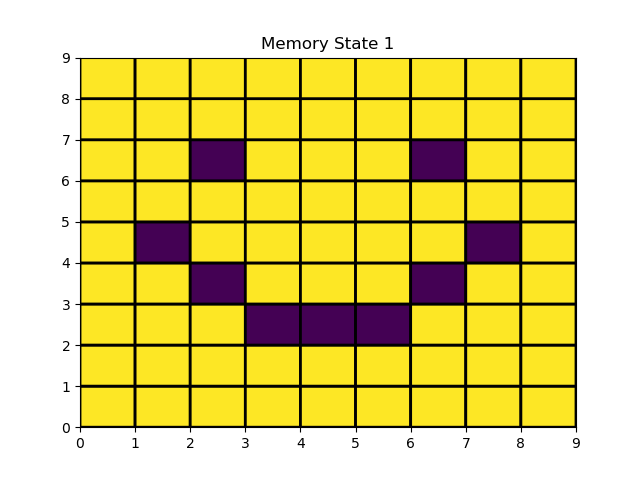
\includegraphics[width=.75\linewidth]{state_9x9_1.png}
	    \end{subfigure}%
	    \begin{subfigure}{.5\linewidth}
	    \centering
	    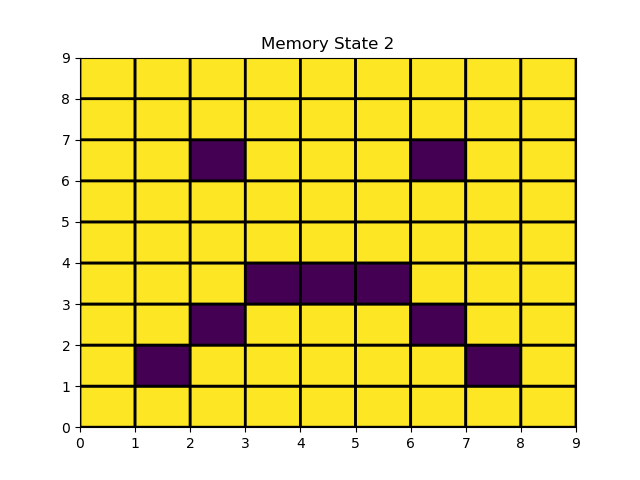
\includegraphics[width=.75\linewidth]{state_9x9_2.png}
	    \end{subfigure}%
	    \caption{Estados de memoria de una red $9 \times 9$ ($N = 81$).}
	    \label{faces}
	\end{figure}
	\\
	\\
    Como procedimiento se realizarán 11 simulaciones a una temperatura fija $T$, todas partiendo del mismo estado inicial aleatorio. En total cada simulación contará con 100000 steps de Montecarlo y se tomará únicamente la información del estado final tras todos los pasos.
    \\
    Para $T = 0$ (en ausencia de ruido) los resultados están representados en la figura de la izquierda de \ref{Mattis-Low-T}. Cada cuadro representa el estado final de la red tras los 100000 steps de una simulación distinta, salvo el cuadro que se encuentra en la esquina superior izquierda, que representa el estado inicial de cada una de las simulaciones. En concreto, para el caso $T = 0$ se observa que todas las simulaciones convergen al mismo estado estable, correspondiente con el estado de memoria de la cara feliz. Éste equivale a uno de los estados de Mattis, para encontrar los otros 3 será necesario irse a una segunda tanda de simulaciones.
	\begin{figure}
	    \centering
	    \begin{subfigure}{.45\textwidth}
	    \centering
	    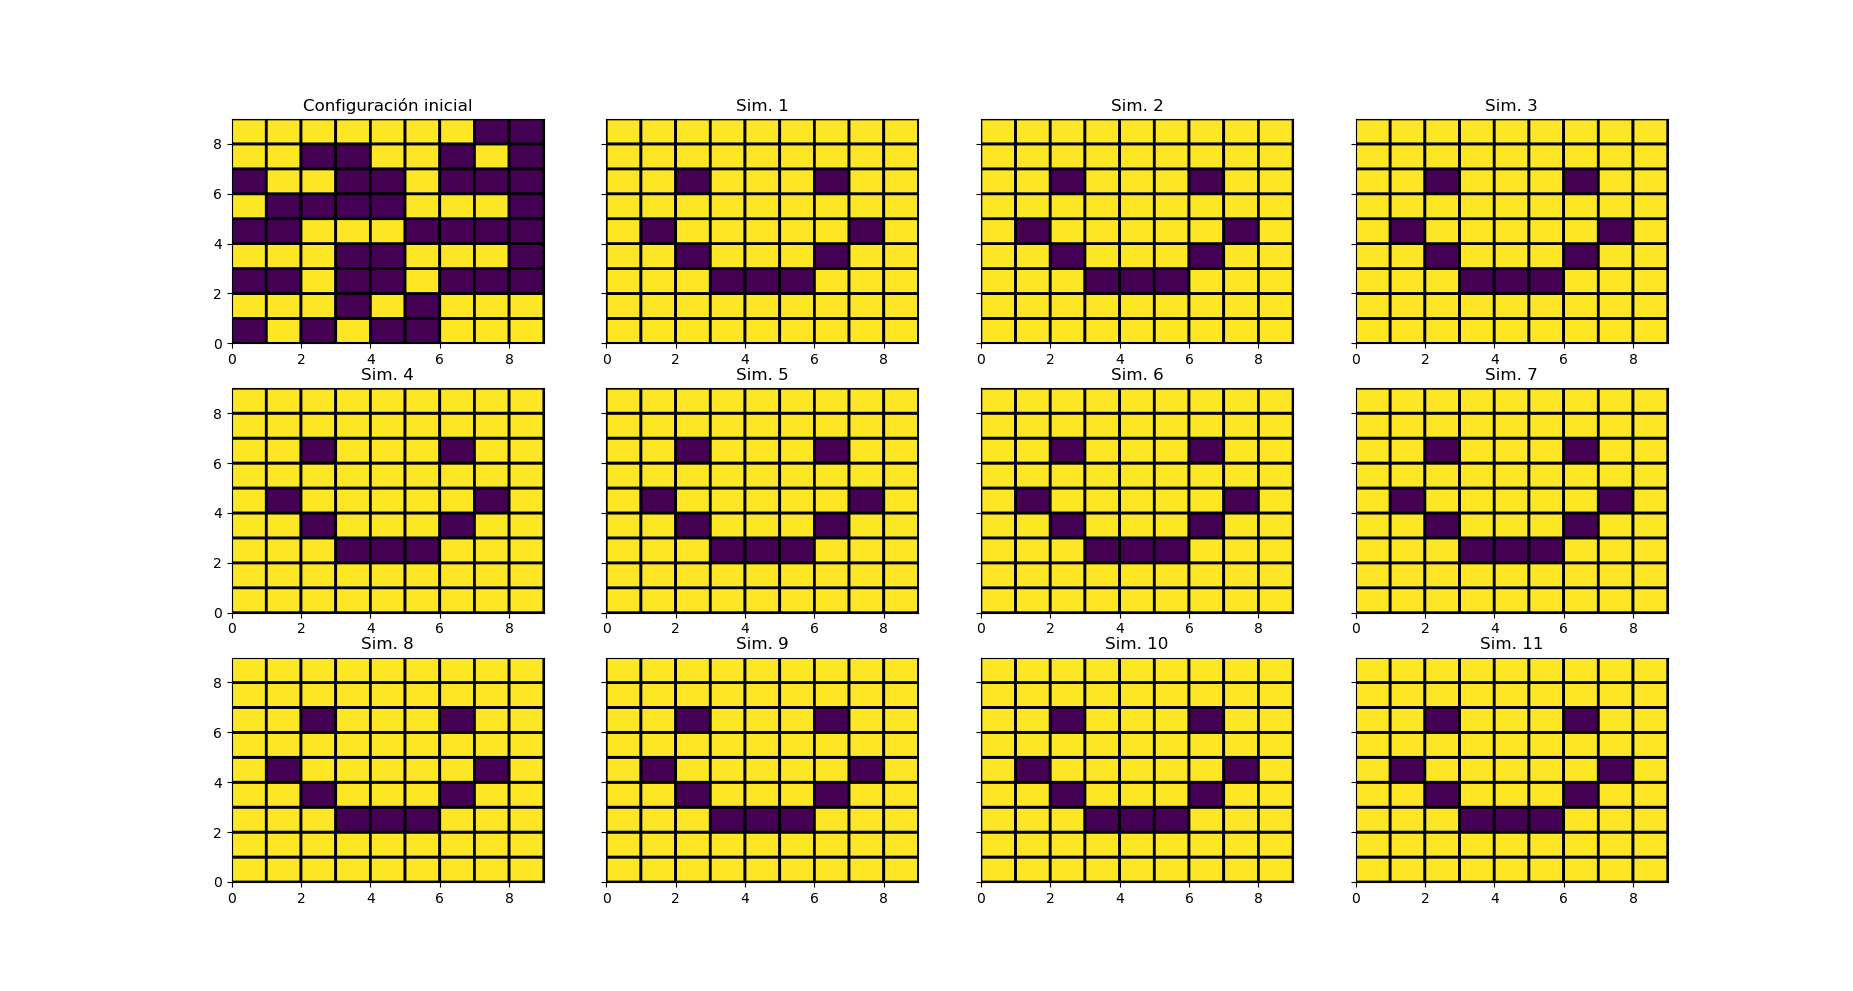
\includegraphics[width=\linewidth]{9x9_T=0.png}
	    \end{subfigure}%
	    \begin{subfigure}{.45\linewidth}
	    \centering
	    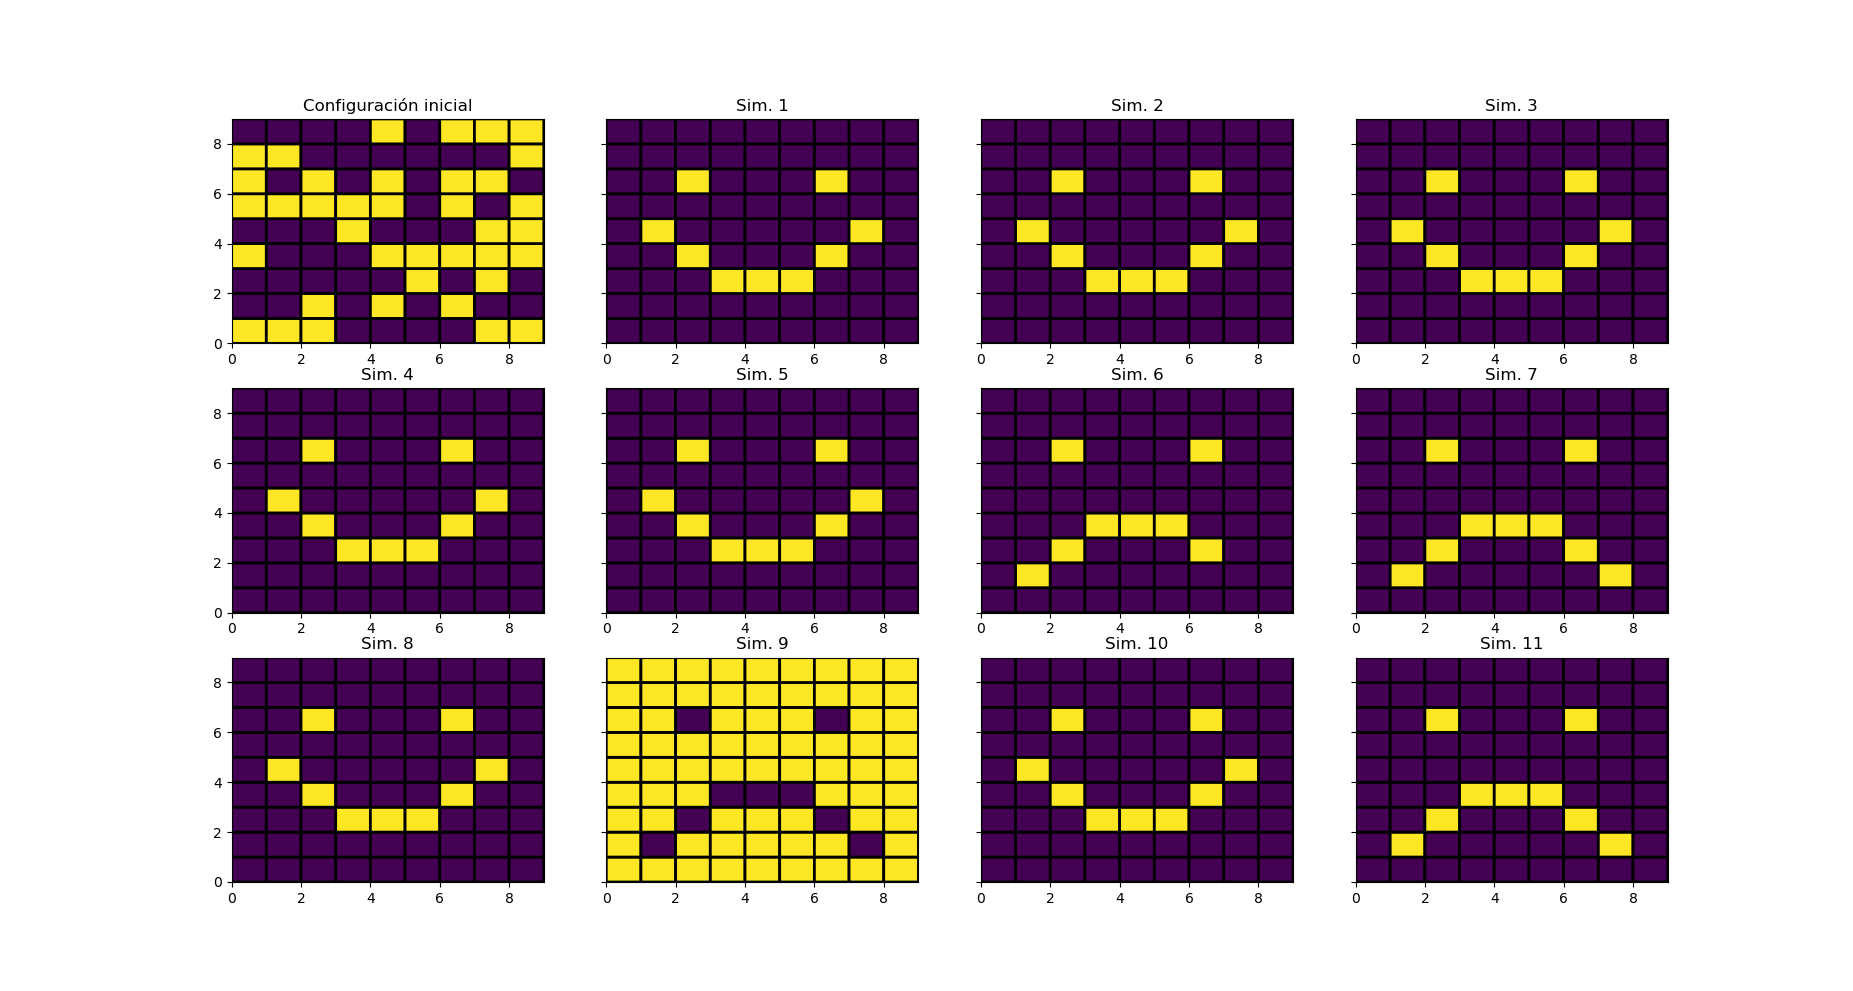
\includegraphics[width=\linewidth]{9x9_T=0,2.png}
	    \end{subfigure}%
	    \caption{Estado final de 11 simulaciones de Montecarlo de 100000 steps a partir de un estado inicial aleatorio (arriba a la izquierda para cada figura). A la izquierda se toma $T = 0$ y a la derecha $T = 0.2$.}
	    \label{Mattis-Low-T}
	\end{figure}
	En la parte derecha de \ref{Mattis-Low-T} se muestran las 11 simulaciones (más el estado inicial) para $T = 0.2$. Aquí sí se ve que existe mayor disparidad con los estados finales. No sólo aparece la cara triste en una de las simulaciones, si no que en el resto la red converge a los estados equivalentes a \ref{faces} al invertir todos los espines. En total todos estos suman 4 estados de Mattis ($2K$) que equivalen a mínimos globales de la energía del Hamiltoniano (\ref{HIsing}).
	\begin{figure}
	    \centering
	    \begin{subfigure}{.45\textwidth}
	    \centering
	    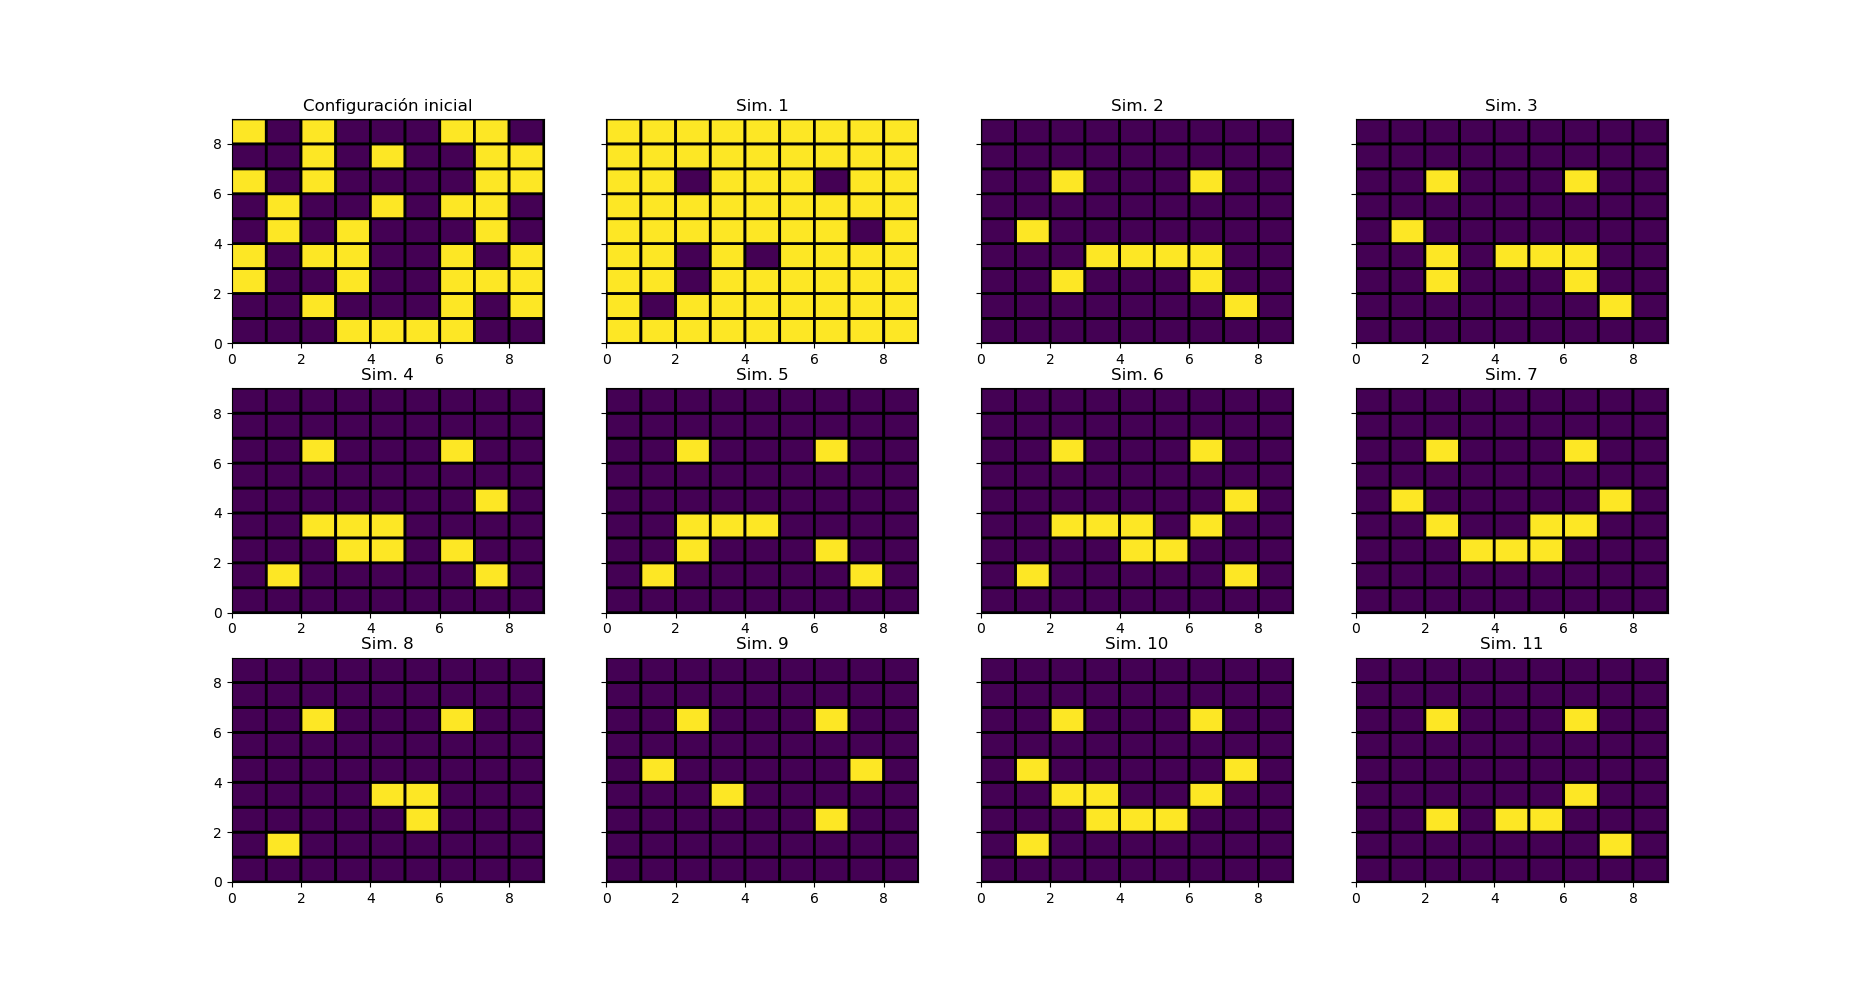
\includegraphics[width=\linewidth]{9x9_T=0,5.png}
	    \end{subfigure}%
	    \begin{subfigure}{.45\linewidth}
	    \centering
	    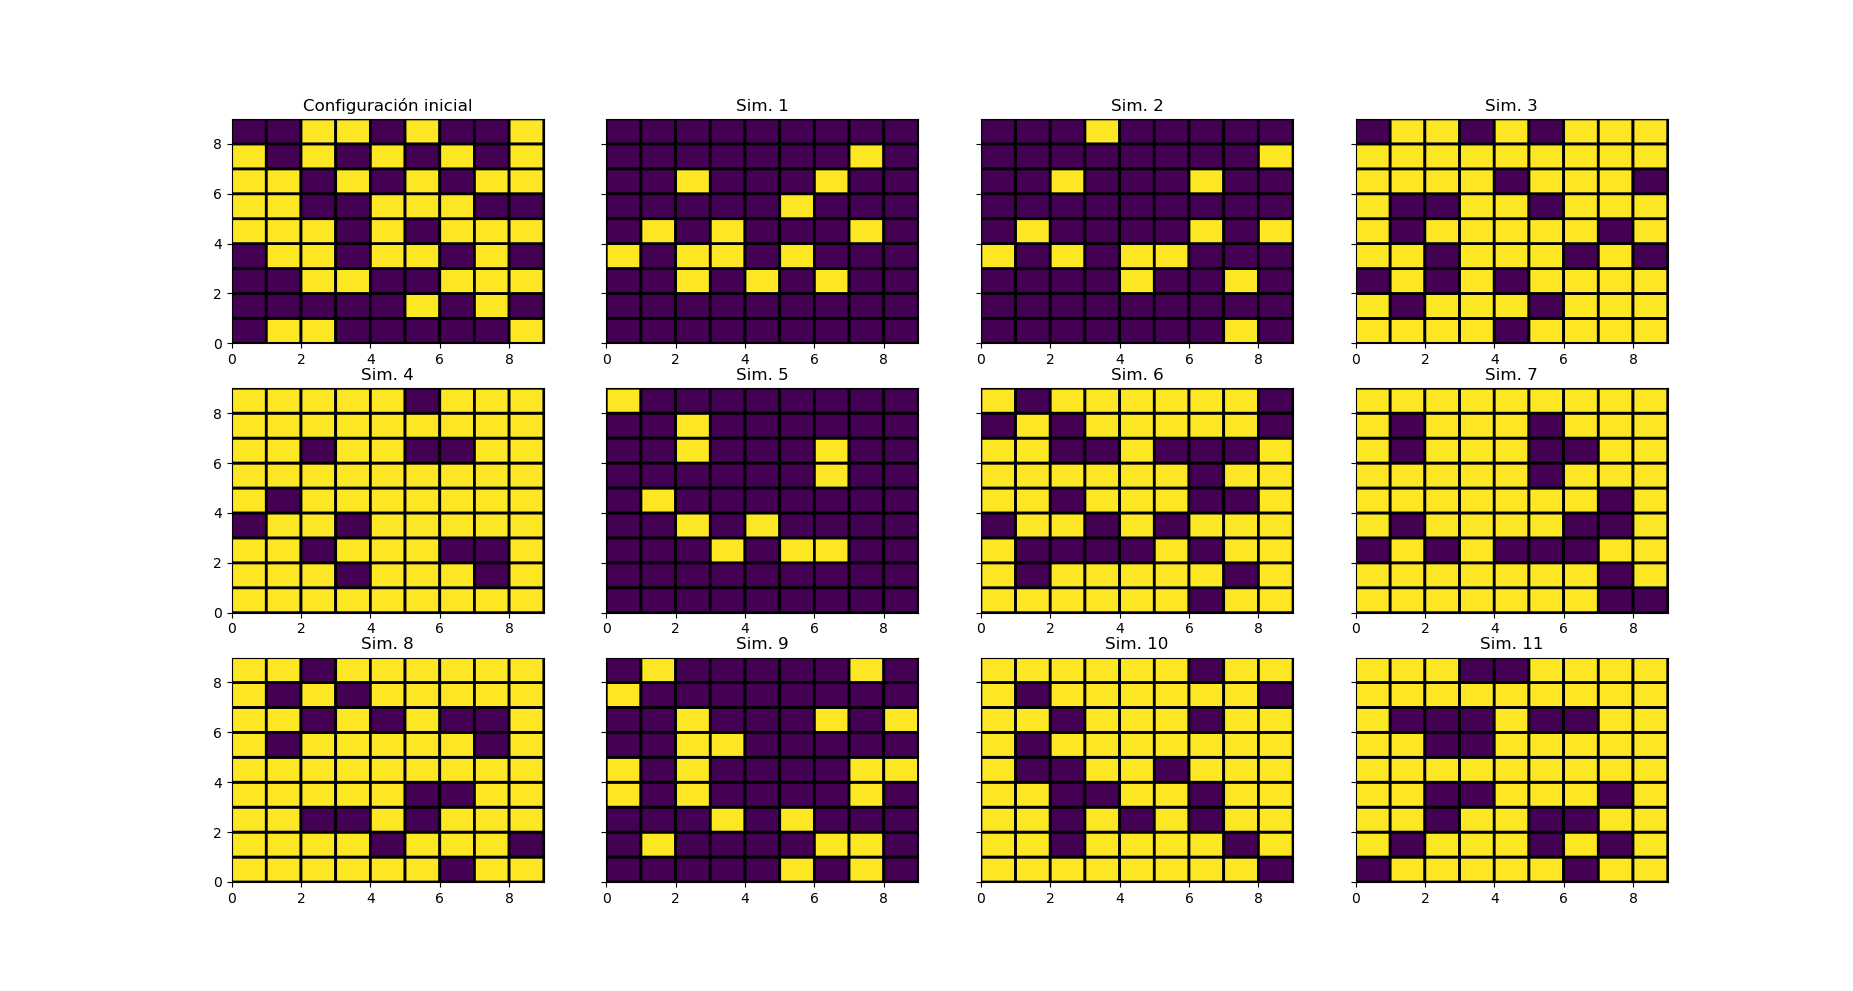
\includegraphics[width=\linewidth]{9x9_T=1,2.png}
	    \end{subfigure}%
	    \caption{Estado final de 11 simulaciones de Montecarlo de 100000 steps a partir de un estado inicial aleatorio (arriba a la izquierda para cada figura). A la izquierda se toma $T = 0.5$ y a la derecha $T = 1.2$.}
	    \label{Mattis-High-T}
	\end{figure}
	\\
	\\
	Los efectos del ruido aprecen expresados en \ref{Mattis-High-T}. A la izquierda se ha simulado con $T - 0.5$ mientras que a la derecha se ha hecho lo propio con $T = 1.2$. Se aprecia que para el caso de las simulaciones con menor ruido las redes siguen convergiendo a un entorno cercano de los mínimos dictados por los estados de memoria, aunque con grandes fluctuaciones. Para  $T = 1.2$ se aprecia que la red es ya incapaz de converger a ningún estado de memoria, decimos entonces que pertenece a la región caótica ($T > T_{c} = 1$, según el análisis de campo medio).
	\subsection{Overlap como parámetro de orden para la transición de fase}
	El \textit{overlap}, o solapamiento, de un estado de la red con cada uno de los estados de memoria ha sido definido al tratar campo medio. Por cuestiones prácticas la manera en la que se calculará el overlap (con el estado de memoria $\mu$) en está sección será mediante la expresión:
	\begin{equation}
	    m^{\mu} = \frac{1}{N} \left| \sum_{i=1}^{N} \langle S_{i} \rangle \mathcal{P}^{\mu}_{i}  \right|
	    \label{overlap-Montecarlo}
	\end{equation}
	Donde $\langle S_{i} \rangle$ es el valor medio del espín $i$. Para calcular este valor medio se realizará en cada simulación 100000 steps de Montecarlo para permitir al sistema alcanzar el equilibrio. Una vez ésto se haya conseguido se realizarán otros 100000 steps para cuantificar esta magnitud, de modo que:
	\begin{equation}
	    \langle S_{i} \rangle = \frac{1}{\text{Número de steps}} \sum_{k=1}^{\text{Número de steps}} S_{i}^{(k)}
	\end{equation}
	El overlap (\ref{overlap-Montecarlo}) se utilizará como parámetro de orden para intentar identificar la transición de fase de la región con memoria a la región caótica al pasar la temperatura crítica $T_{c} = 1$. Para ello se representa para redes con distintos tamaños y con $K = 1$ el overlap con el único estado de memoria en \ref{FSS-Overlap}.
	\begin{figure}
	    \centering
	    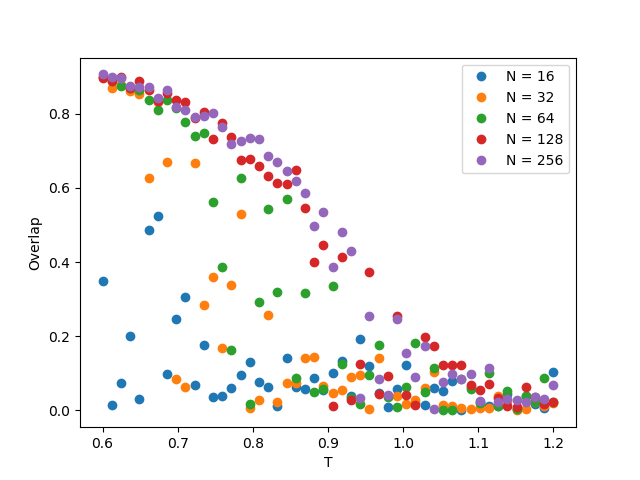
\includegraphics[width=.45\linewidth]{Overlap_FSS.png}
	    \caption{Overlap (\ref{overlap-Montecarlo}) en función de la temperatura para distintos tamaños de la red. En todos los casos se ha tomado sólo un estado de memoria.}
	    \label{FSS-Overlap}
	\end{figure}
	\\
	Se identifica en esta figura un claro descenso del overlap conforme aumenta la temperatura. Se pueden diferenciar ambas regiones (la de memoria y la caótica) con cierto rango de ambigüedad debido a que en ningún punto se puede afirmar que se alcance el límite termodinámico. Una de las hipótesis que se barajan es que en el límite $N \to \infty$ exista una no analiticidad de $m^{\mu}$ en $T = 1$ debido a la variación en la pendiente que se deja entrever en \ref{FSS-Overlap}, esto conllevaría que la transición de fase que sufre la red es de segundo orden.
	\subsection{Estados metaestables}
	Para finalizar en esta subsección se pretenden encontrar estados metaestables. Éstos estados equivalen a mínimos locales del Hamiltoniano que no se corresponden con ningún estado de memoria. Se corresponen con estados estables que, en el caso de estados de memoria ortogonales, tienen un overlap no nulo con cada uno de los $K$ estados $\{\mathcal{P}^{\mu}\}$.
	\\
	El procedimiento que se seguirá para encontrarlos será representar el módulo de la \text{magnetización}, así como la energía de la red de espines a lo largo de toda su evolución, para comprobar que ésta ha caído en un mínimo estable. La magnetización se define como el valor medio de los espines de la red, con lo que su módulo es:
	\begin{equation}
	    \left|M(\{S\})\right| = \frac{1}{N} \left| \sum_{i=1}^{N} S_{i} \right|
	\end{equation}
	La razón por la que a su vez se representa la energía es para asegurarse de la convergencia del sistema a uno de estos mínimos locales, pues puede darse el caso de que la red fluctúe entre dos estados con misma magnetización.
	\\
	En esta ocasión se utilizan tres estados de memoria ortogonales para una red $10 \times 10$ ($N = 100$). Estos estados se encuentran representados en \ref{ortogonal-states}. Los estados metaestables se han encontrado para temperaturas bajas ($T = 0$, $T = 0.1$ y $T = 0.2$), puesto que al ser mínimos locales cualquier fluctuación lo suficientemente grnde debida al ruido puede sacar a la red del pozo de potencial. Los resultados se representan en las figuras \ref{meta-T=0}, \ref{meta-T=0.1} y \ref{meta-T=0.2} de la página siguiente.
	\\
	Estos estados tienen overlap no nulo con cada cada uno de los estados de memoria, lo cual confirma su carácter metaestable. En la figura \ref{meta-overlap} se representan los overlaps del estado obtenido tras la simulación de \ref{meta-T=0} (a $T = 0$).
	\begin{figure}
	    \centering
	    \begin{subfigure}{.3\textwidth}
	    \centering
	    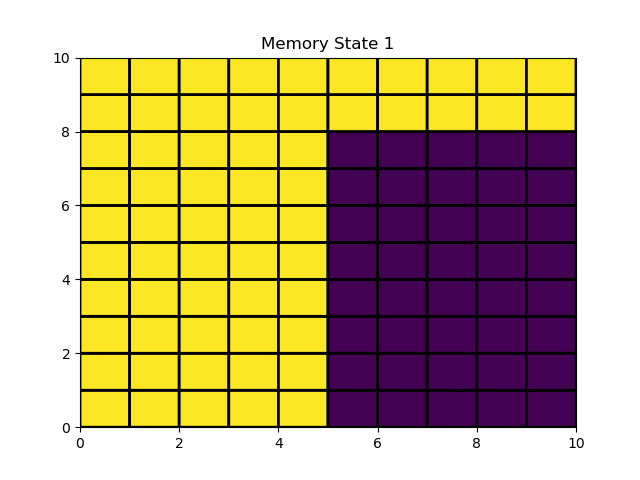
\includegraphics[width=\linewidth]{state_10x10_1.png}
	    \end{subfigure}%
	    \begin{subfigure}{.3\linewidth}
	    \centering
	    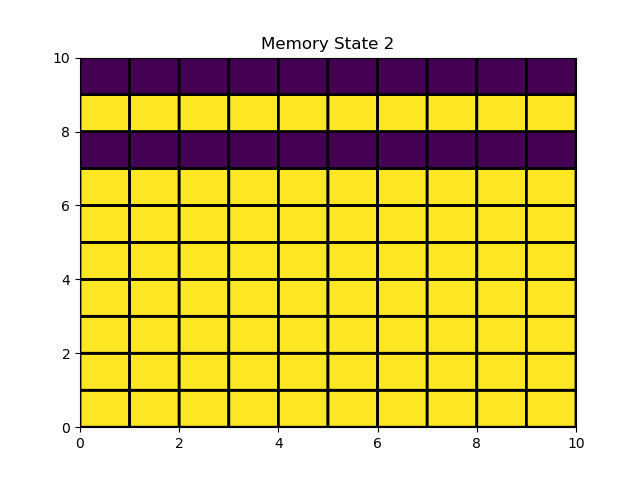
\includegraphics[width=\linewidth]{state_10x10_2.png}
	    \end{subfigure}%
	    \begin{subfigure}{.3\textwidth}
	    \centering
	    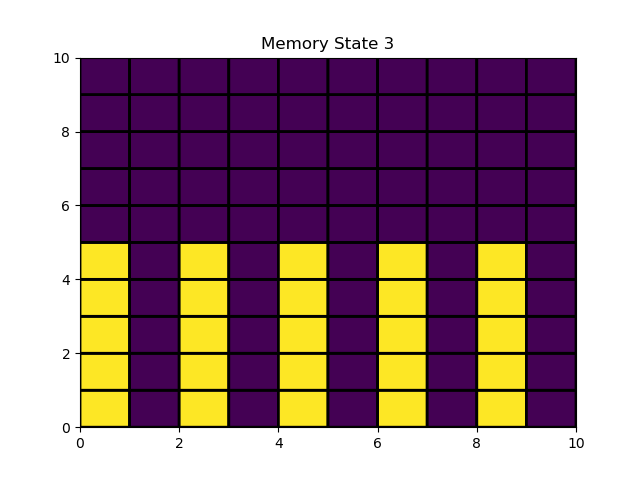
\includegraphics[width=\linewidth]{state_10x10_3.png}
	    \end{subfigure}%
	    \caption{Estados de memoria ortogonales de una red $10 \times 10$ ($N = 100$).}
	    \label{ortogonal-states}
	\end{figure}
	\begin{figure}
	    \centering
	    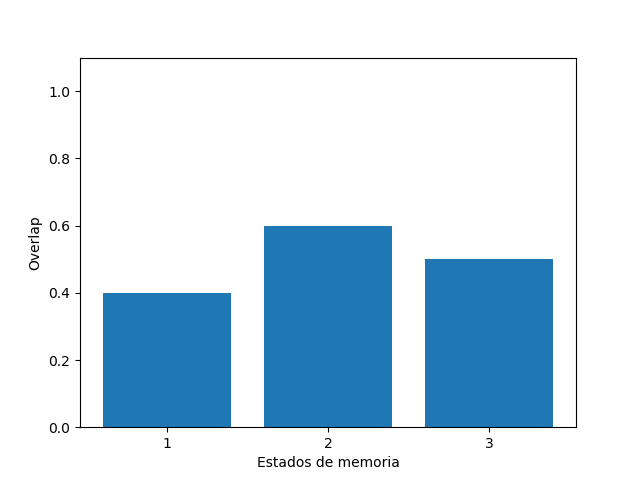
\includegraphics[width=.45\linewidth]{Metastable_overlap.png}
	    \caption{Overlap con cada estado de memoria del estado metaestable obtenido en la simulación \ref{meta-T=0}.}
	    \label{meta-overlap}
	\end{figure}
	\newpage
	\begin{figure}[H]
	    \centering
	    \begin{subfigure}{.45\textwidth}
	    \centering
	    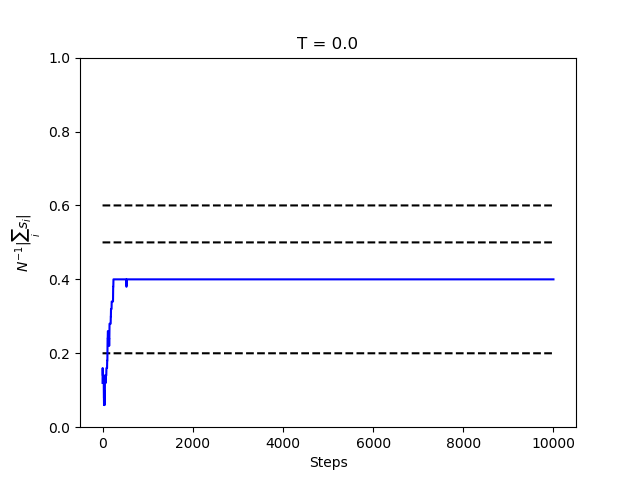
\includegraphics[width=\linewidth]{magnet_meta_T=0,0.png}
	    \end{subfigure}%
	    \begin{subfigure}{.45\linewidth}
	    \centering
	    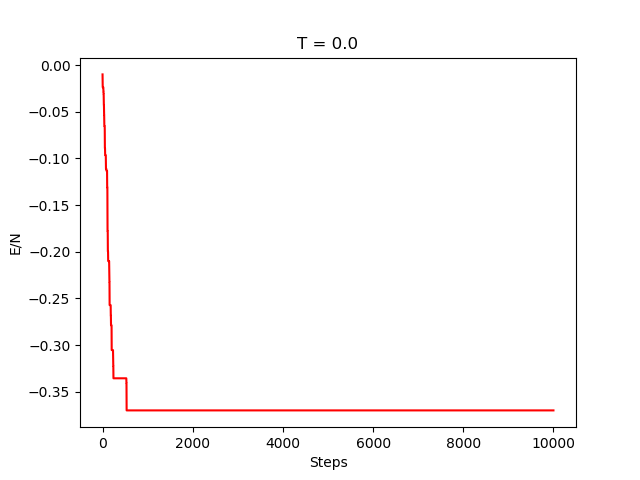
\includegraphics[width=\linewidth]{ener_meta_T=0,0.png}
	    \end{subfigure}%
	    \caption{Evolución de la magnetización (izquierda) y la energía (derecha) para la misma simulación de Montecarlo a $T = 0$. Las líneas negras discontinuas de la izquierda representan las magnetizaciones de los estados de memoria.}
	    \label{meta-T=0}
	\end{figure}
	\begin{figure}[H]
	    \centering
	    \begin{subfigure}{.45\textwidth}
	    \centering
	    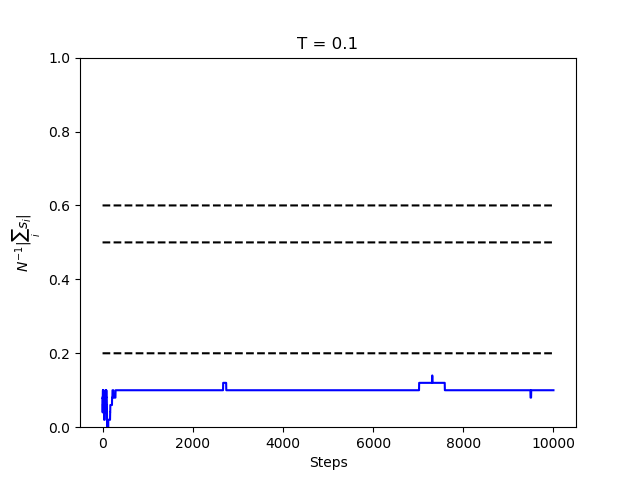
\includegraphics[width=\linewidth]{magnet_meta_T=0,1.png}
	    \end{subfigure}%
	    \begin{subfigure}{.45\linewidth}
	    \centering
	    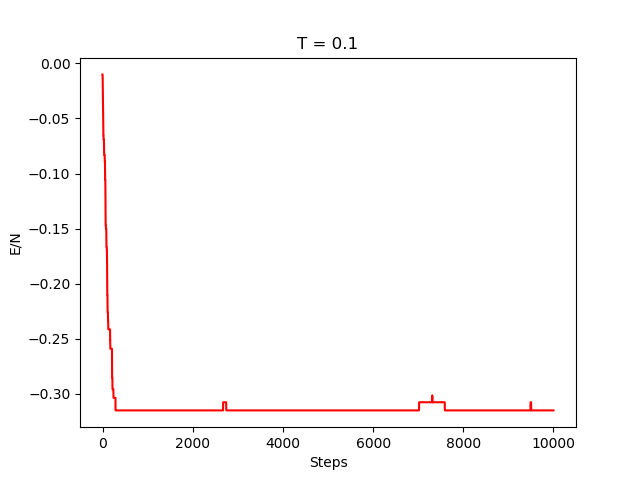
\includegraphics[width=\linewidth]{ener_meta_T=0,1.png}
	    \end{subfigure}%
	    \caption{Evolución de la magnetización (izquierda) y la energía (derecha) para la misma simulación de Montecarlo a $T = 0.1$. Las líneas negras discontinuas de la izquierda representan las magnetizaciones de los estados de memoria.}
	    \label{meta-T=0.1}
	\end{figure}
	\begin{figure}[H]
	    \centering
	    \begin{subfigure}{.45\textwidth}
	    \centering
	    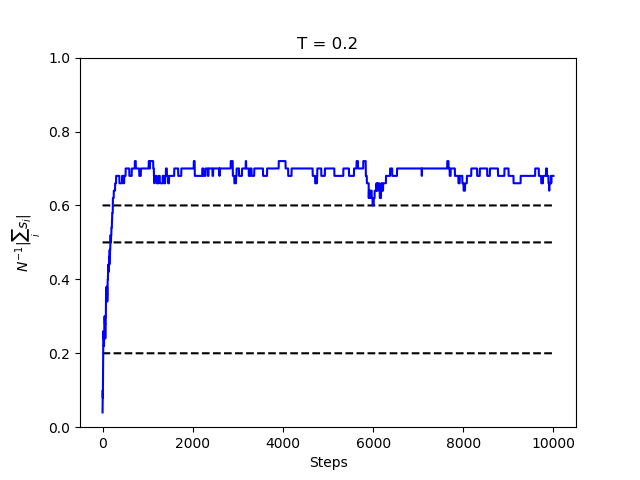
\includegraphics[width=\linewidth]{magnet_meta_T=0,2.png}
	    \end{subfigure}%
	    \begin{subfigure}{.45\linewidth}
	    \centering
	    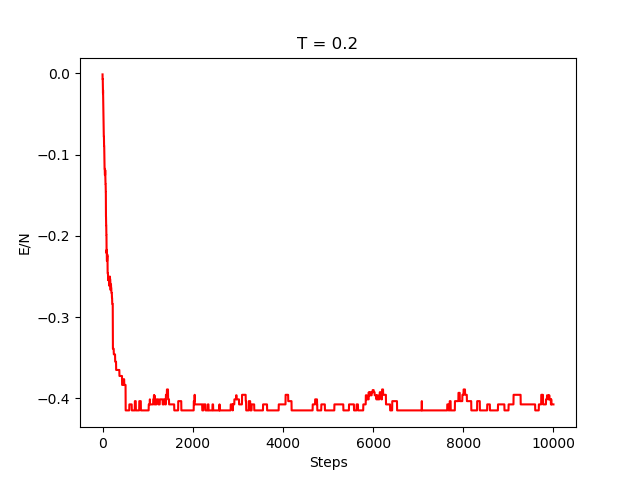
\includegraphics[width=\linewidth]{ener_meta_T=0,2.png}
	    \end{subfigure}%
	    \caption{Evolución de la magnetización (izquierda) y la energía (derecha) para la misma simulación de Montecarlo a $T = 0.2$. Las líneas negras discontinuas de la izquierda representan las magnetizaciones de los estados de memoria.}
	    \label{meta-T=0.2}
	\end{figure}
	%\begin{figure}
	    %\centering
	    %\begin{subfigure}{.33\textwidth}
	    %\centering
	    %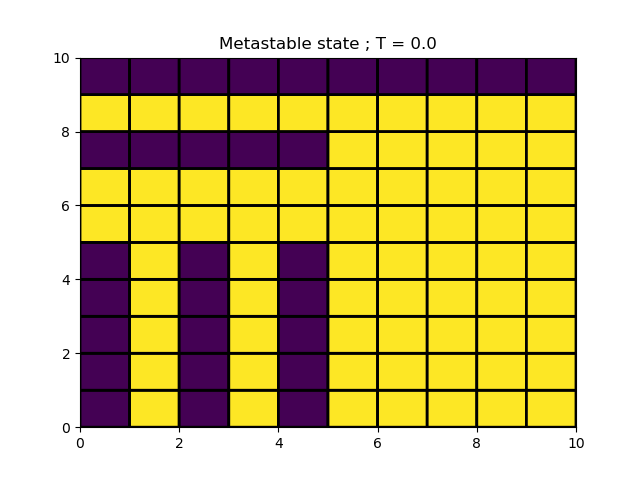
\includegraphics[width=\linewidth]{meta_T=0,0.png}
	    %\end{subfigure}%
	    %\begin{subfigure}{.33\linewidth}
	    %\centering
	    %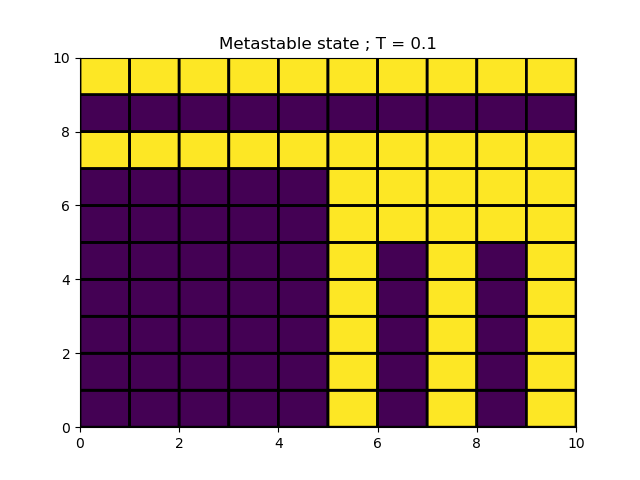
\includegraphics[width=\linewidth]{meta_T=0,1.png}
	    %\end{subfigure}%
	    %\begin{subfigure}{.33\textwidth}
	    %\centering
	    %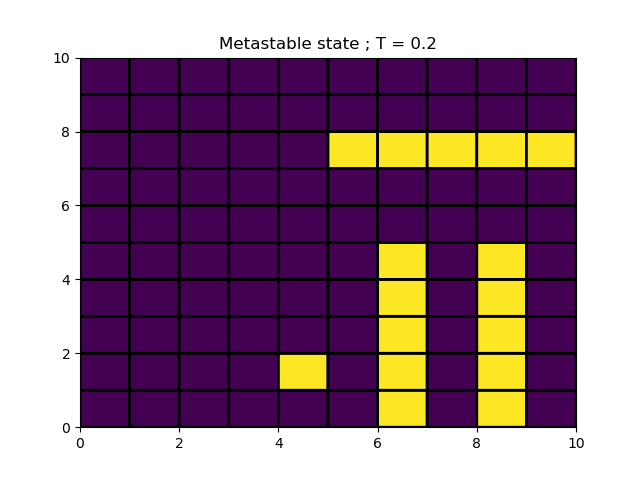
\includegraphics[width=\linewidth]{meta_T=0,2.png}
	    %\end{subfigure}%
	    %\caption{Estados metaestables surgidos de las simulaciones representadas en \ref{meta-T=0}, %\ref{meta-T=0.1} y \ref{meta-T=0.2}, respectivamente.}
	 %   \label{metastable-states}
	%\end{figure}
	
	\subsection{Conclusiones}
	De los resultados de todas las subsecciones anteriores se puede afirmar de manera bastante rotunda la veracidad del análisis de campo medio realizado en las primeras secciones del texto. Se ha comprobado la existencia de los $2K$ estados de Mattis sin problema alguno, así como se ha visto el efecto que tiene el ruido sobre la memoria de la red. También se ha mostrado el overlap con los estados de memoria como un muy buen parámetro de orden para cuantificar la transición de fase de memoria-caos, aunque simulaciones con redes más grandes son necesarias para una determinación más precisa de las propiedades de ésta. Por último, la existencia de estados metaestables ha sido comprobada sin dejar lugar a dudas, siendo la aparición de estos mínimos locales una de las consecuencias más anti-intuitivas del modelo.
	
	\section{Ecuación de Langevin para la dinámica de los espines}
	En la sección 1, hicimos un breve comentario sobre la dinámica de los espines, donde establecimos que si un estado es parcialmente similar a aquellos que forman el patrón, la dinámica llevará los espines a dichos estados estacionarios. Feigelman et. al. \cite{feigelman86} proponen la ecuación de Langevin que gobierna esta dinámica. 
	
	El primer paso que tomaremos será añadir una modificación al hamiltoniano en forma de un término con un nuevo potencial $V(\sigma_i)$ para cada espín; lo que en realidad nos interesa no es este potencial en sí, si no su derivada, cuyo fin se hará vigente en las ecuaciones del movimiento. Nuestro hamiltoniano es entonces:
	\begin{equation}
	H = \sum_i V(\sigma_i) + \frac{1}{2}\sum_{i}\sum_{j\neq i}J_{ij}\sigma_i\sigma_j
	\label{Hfeigelman}
	\end{equation}
	
	Las ecuaciones de movimiento dadas por \eqref{Hfeigelman} serán equivalentes a las ecuaciones de Langevin para la evolución de los espines $\sigma_i$. Estas son \cite{feigelman86}:
	\begin{equation}
	\frac{\partial\sigma_i}{\partial t} = -\frac{\partial V(\sigma_i)}{\partial\sigma_i} + \sum_j J_{ij}\sigma_j + h_i\sigma_i + \xi_i(t)
	\label{langevin}
	\end{equation}
	En esta dinámica gobernada por \eqref{langevin} los patrones serán estados estables con un rango de atracción en el espacio de configuración, de modo que si un estado inicial $\tilde{\sigma_i}$ es parcialmente similar a uno de los estados estacionarios que $\sigma_i$ conforman el patrón, la dinámica llevará $\tilde{\sigma_i}$ a $\sigma_i$; este es el mecanismo mediante el cual la red recuerda el patrón.\\
	
	Estudiemos ahora los distintos términos de \eqref{langevin}. En estas ecuaciones aparece la derivada del potencial que hemos introducido anteriormente, ${\partial V(\sigma_i)}/{\partial \sigma_i}$. La razón de ser de este término es asegurar que (al menos casi siempre) el valor dado por esta ecuación para los espines sea $\sigma_i=\pm 1$.
	\begin{center}
	    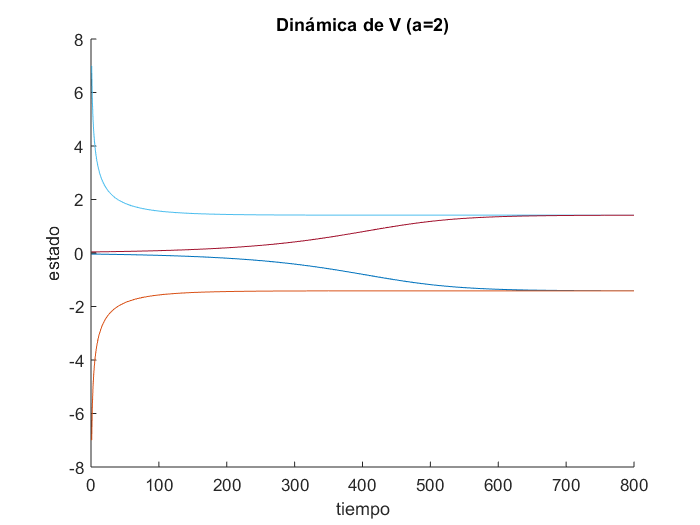
\includegraphics[scale=0.5]{potencial}\\
	  \begin{small}
	  Dinámica del potencial con convergencia en $\sigma=\pm2$. Se ha usado un valor diferente a 1 (el usado en el trabajo) para exponer el comportamiento de dicha dinámica de un modo más general.
	\end{small}
	\end{center}
	La elección de este potencial es $V(\sigma_i)=\lambda\left(\sigma_i^2-1\right)^2$. Cuando el potencial toma esta forma, resolver la dinámica nos lleva al resultado:
	\begin{displaymath}
	\sigma_i = \frac{\pm 1}{\sqrt{1-e^{-2\lambda t}}} \xrightarrow[t \rightarrow \infty]{}\pm 1
	\end{displaymath}
	es decir, vemos que en el límite asintótico de tiempos infinitos, los valores de los espines son los esperados, $\pm 1$. La elección de este potencial está basado en imponer las condiciones de convergencia, de modo que si se utilizan otros potenciales (por ejemplo cuadráticos en vez de cuárticos) se puede comprobar que este comportamiento puede no replicarse, por eso es necesario introducir el potencial usado para que la dinámica sea coherente con las reglas del modelo. Por otro lado, el parámetro $\lambda$ debe ser positivo; en el caso de que fuera negativo los espines convergerían a $0$, y en el caso de que fuera $\lambda = 0$ (no hay potencial) los valores crecen sin control. Pero también necesitamos que tenga valores grandes respecto a $1$: se puede comprobar que el valor al que convergen los espines para un valor de $\lambda$ dado es:
	\begin{displaymath}
	|\sigma_i|_{estacionario}=\sqrt{1 + \frac{1}{\lambda}}
	\end{displaymath}
	por tanto necesitamos que, como mínimo, $\lambda >> 1$, o preferiblemente $\lambda\rightarrow\infty$. Este hecho cobrará importancia cuando posteriormente llevemos a cabo simulaciones numéricas con la dinámica gobernada por \eqref{langevin}.

    En efecto, si consideramos que los espines han convergido al patrón $\mathcal{P}^\nu_i$, tenemos que $\sigma_i = \sqrt{1 + \frac{1}{\lambda}} \mathcal{P}^\nu_i$. Imponiendo que el estado sea estacionario en \eqref{langevin}, a $T = 0$ obtenemos:

	\begin{equation*}
	\sum_{j=1}^N J_{ij}\sigma_j - \lambda(\sigma_i^2-1)\sigma_i = \sqrt{1 + \frac{1}{\lambda}} \left( \sum_{\mu=1}^K \mathcal{P}^\mu_i \frac{1}{N} \sum_{j=1}^N \mathcal{P}^\mu_j \mathcal{P}^\nu_j  - \mathcal{P}^\mu_i \right) = 0
	\end{equation*} 
	
	Por otro lado, hemos introducido el ruido blanco gaussiano $\xi_i(t)$, que satisface $\left<\xi_i(t)\xi_j(t')\right>=2T\delta_{ij}\delta(t-t')$, dónde $T$ es la temperatura efectiva que se introduce en el modelo de Hopfield generalizado que hemos comentado en la sección 2, como representante del ruido de fondo en el sistema.
	
	Por último, tomaremos como pesos de interacción $J_{ij}$ los definidos en \eqref{Jint}. Son la forma más simple que pueden tomar para reproducir la dinámica deseada. 
	
	En el siguiente apartado utilizaremos esta dinámica para, mediante métodos numéricos, examinar como la red (a una temperatura fija dada $T$) evoluciona hacia un patrón dado externamente desde un estado inicial aleatoriamente desordenado, siguiendo la dinámica dada por \eqref{langevin}. En la figura \ref{ejemplo} se muestra un ejemplo.
	\begin{center}
		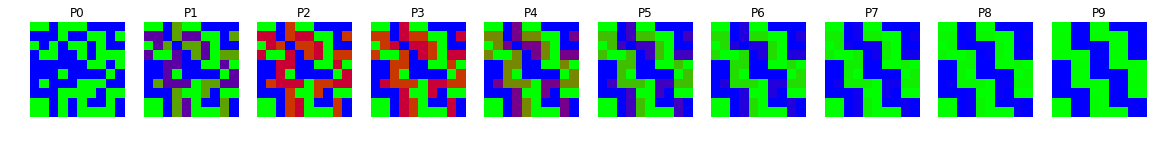
\includegraphics[width=16cm]{pasos.png}
		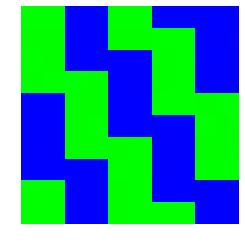
\includegraphics[width=4cm]{final.png} 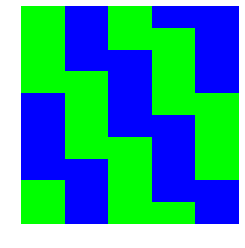
\includegraphics[width=4cm]{patron.png}
		\captionof{figure}{Arriba, la evolución de la red desde el estado desordenado P0 hasta el estado final P9. Abajo, el estado final de la red (izquierda) junto al patrón almacenado (derecha). Vemos que la red ha conseguido reproducir exitosamente el patrón.} \label{ejemplo}
	\end{center}
	\subsection{Simulación numérica de la dinámica}
	%En esta sección presentamos una simulación numérica llevada a cabo en Python, utilizando el paquete \verb|neurodynex| proporcionado en \cite{neurodyn-ex}.
	Anteriormente se han expuesto imágenes resultantes de la simulación de la ecuación de Langevin en python usando el paquete \verb|neurodynex| proporcionado en \cite{neurodyn-ex}. En esta sección se estudiará la dinámica del sistema en profundidad utilizando Matlab.
	
	Para poder tratar el problema de este modo, el primer paso que hemos de tomar es traducir la ecuación diferencial \eqref{langevin} a una de diferencias finitas. Como ya comentamos en la sección 1, la dinámica de la red neuronal evoluciona por pasos temporales finitos, la dinámica de decaimiento exponencial debe ser rápida (en tiempos de orden $1$), mientras que la dinámica debida al modelo de Ising debe ser lenta.
	\begin{displaymath}
	\sigma_i(t+dt) - \sigma_i(t) = \left(  -4\lambda(\sigma_i^2 - 1)\sigma_i +  \sum_j J_{ij} \sigma_j + h_i\sigma_i \right) dt + \sqrt{2T}dW
	\end{displaymath}
	Absorbiendo el $4$ en el parámetro $\lambda$ y despejando, obtenemos:
	\begin{equation}
	\sigma_i(t+dt) = g(\sigma_i(t)) = \left(  -\lambda(\sigma_i^2 - 1)\sigma_i +  \sum_j J_{ij} \sigma_j + h_i\sigma_i \right) dt + \sqrt{2T}dW + \sigma_i(t)
	\label{dynfunc}
	\end{equation}
	de forma que $g (\sigma_i(t))$ será la función dinámica que utilicemos en el cálculo. Para convertir la ecuación de Langevin en una ecuación diferencial estocástica, hemos introducido el diferencial estocástico $dW$ cuyos dos primeros momentos (media y desviación) cumplen:
\begin{equation*}
\mu(dW) = 0, \hspace{10mm} \sigma^2(dW) = dt
\end{equation*}

A la hora de calcular los resultados, tenemos que reescalar este termino dW para que la temperatura sea independiente de la elección de $\lambda$, ya que si no, una elección de $\lambda$ pequeño hará que el sistema no responda a temperaturas altas. Dicho escalado será $dW \rightarrow \sqrt{1+\frac{1}{\lambda}}dW$, y así tendremos un comportamiento independiente entre la temperatura y $\lambda$.\\
Por consiguiente, cuando el sistema llegue al equilibrio, dividiremos los estados entre $ \sqrt{1+\frac{1}{\lambda}}$ para recuperar los valores $\pm 1$.\\
A la hora de seleccionar los términos multiplicados por dt, para el primero (el potencial) elegimos un $\lambda$ arbitrario (0.01) y $h_i=\vec{0}$ (para que el sistema evolucione libremente). La elección de $J_{ij}$ es importante, ya que hay que construirla a partir de los patrones que queremos que el sistema memorice. Para esto tenemos que tener en cuenta que existe una cantidad máxima de estados que el sistema puede almacenar sin presentar un estado de memoria caótica (en el cual se pierden los estados almacenados), determinado por la fórmula:
\begin{equation*}
    Q= \frac{L}{ln(L^2)}
\end{equation*}
Una vez tenemos todo preparado, estudiaremos como evoluciona el sistema ante diferente número de patrones y a diferentes T en una red con una longitud de LxL. Para esto queremos recorrer todos los estados iniciales y mediremos la cantidad de estados finales que no coinciden con los esperados, ya que esperamos que los estados estacionarios sean igual a los patrones que hemos usado para construir la matriz $J_{ij}$. Al ser esto computacionalmente muy costoso, elegimos una cantidad suficientemente grande de diferentes estados iniciales de manera aleatoria. Lo cual nos permite visualizar el comportamiento del sistema.\\

Para una red de 8x8, obtenemos:\\
\begin{center}
    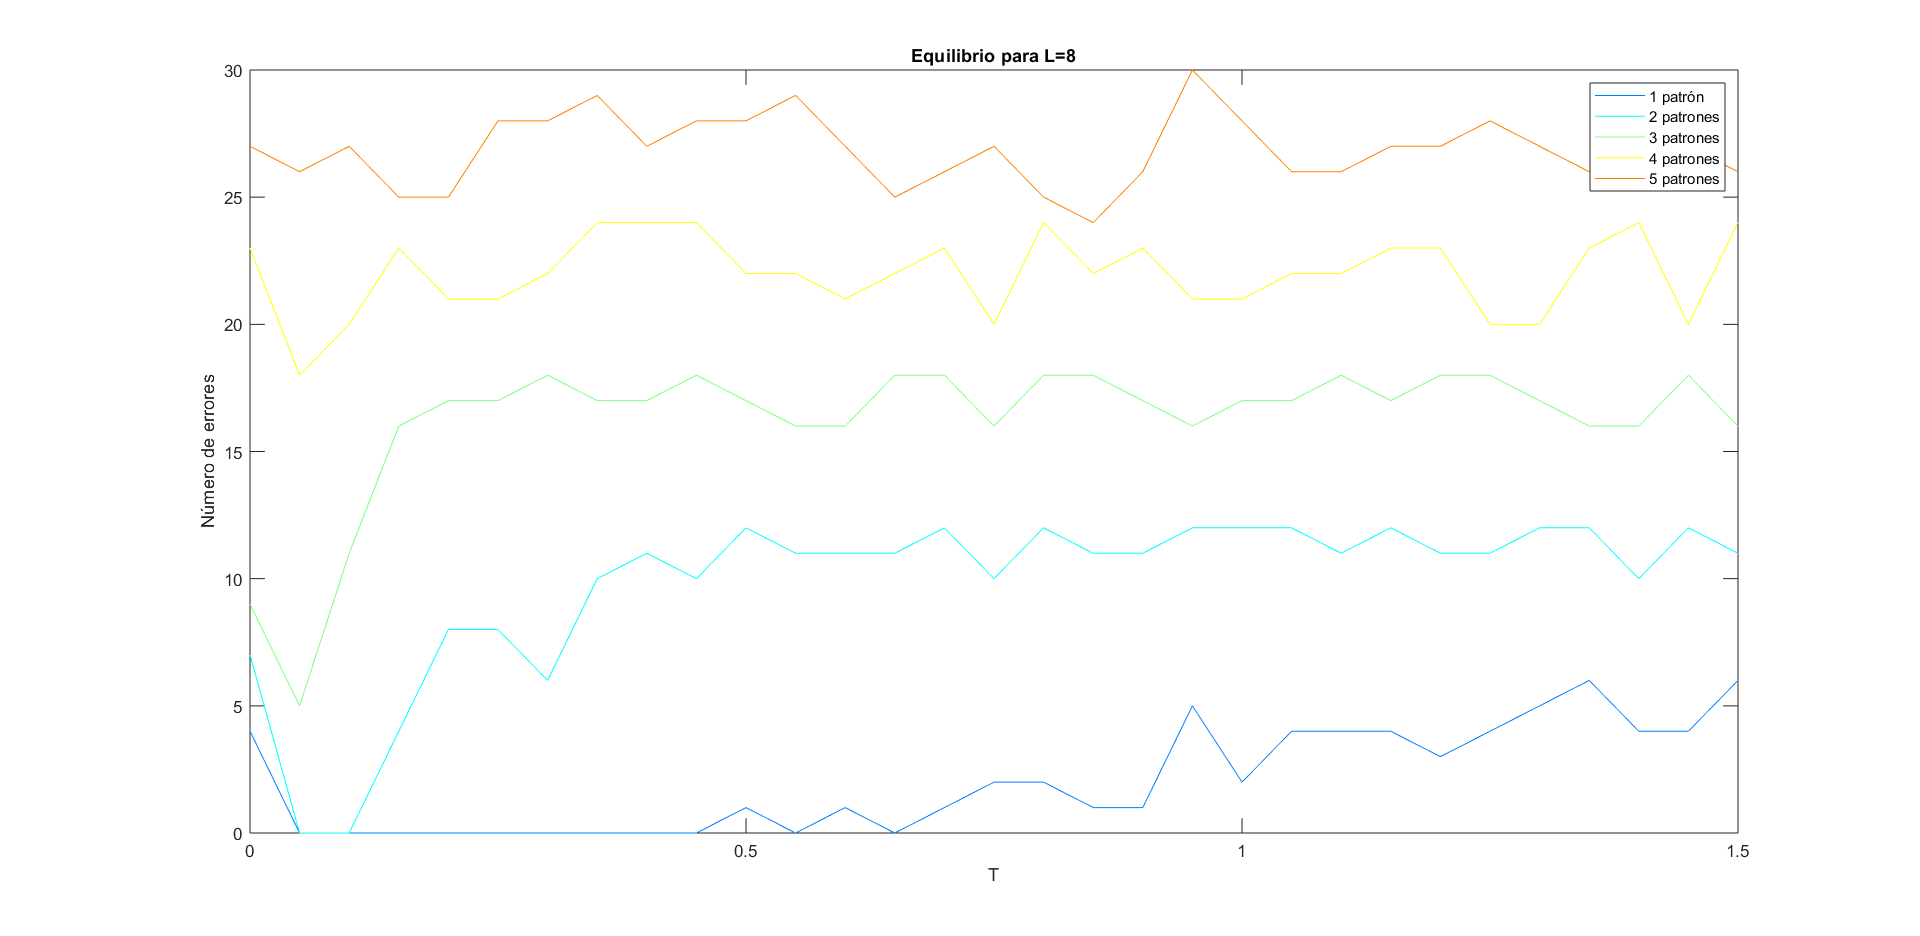
\includegraphics[scale=0.3]{dinamicaL8.png}
\end{center}

Vamos a comentar todo lo que observamos en esta gráfica.\\
En primer lugar, para una red de L=8 el número máximo de patrones que podemos almacenar sin obtener fallos serán dos. Sin embargo, no observamos que esto ocurra para T=0, sino para T no nulas muy pequeñas. Esto ocurre debido a que, si el estado inicial es ortogonal a alguno de los patrones almacenados, todos los términos de la evolución temporal se van a anular y el sistema no evoluciona. Sin embargo, si aplicamos una perturbación muy pequeña, la evolución temporal será diferente de cero y el sistema sí evolucionará como queremos.\\
A medida que aumentamos el número de patrones almacenados en la red, perdemos la capacidad de almacenamiento y el número de errores aumenta para cualquier temperatura. Cuando el número de patrones es muy alto, el sistema no guarda ningún estado de memoria. Esto es debido porque todos los estados iniciales serán ortogonales a alguno de los patrones almacenados y por tanto no hay ningún tipo de evolución. Aún aumentando la temperatura, tampoco se reduce el número de errores. Esto es lo que denominamos régimen caótico de memoria.\\
Por otro lado, tenemos una variación del número de errores medidos en el sistema respecto a la temperatura, donde al aumentar este parámetro lo suficiente, el sistema tiene problemas al alcanzar el estado de equilibrio, produciendo que aumente el número de errores. \textbf{es importante destacar} que para T alta, cada gráfica tiene un número diferente de errores porque se han usado un \textbf{número diferente de estados iniciales}.\\
Vamos a ver también la dinámica para una red mayor, con L=64:\\
\begin{center}
     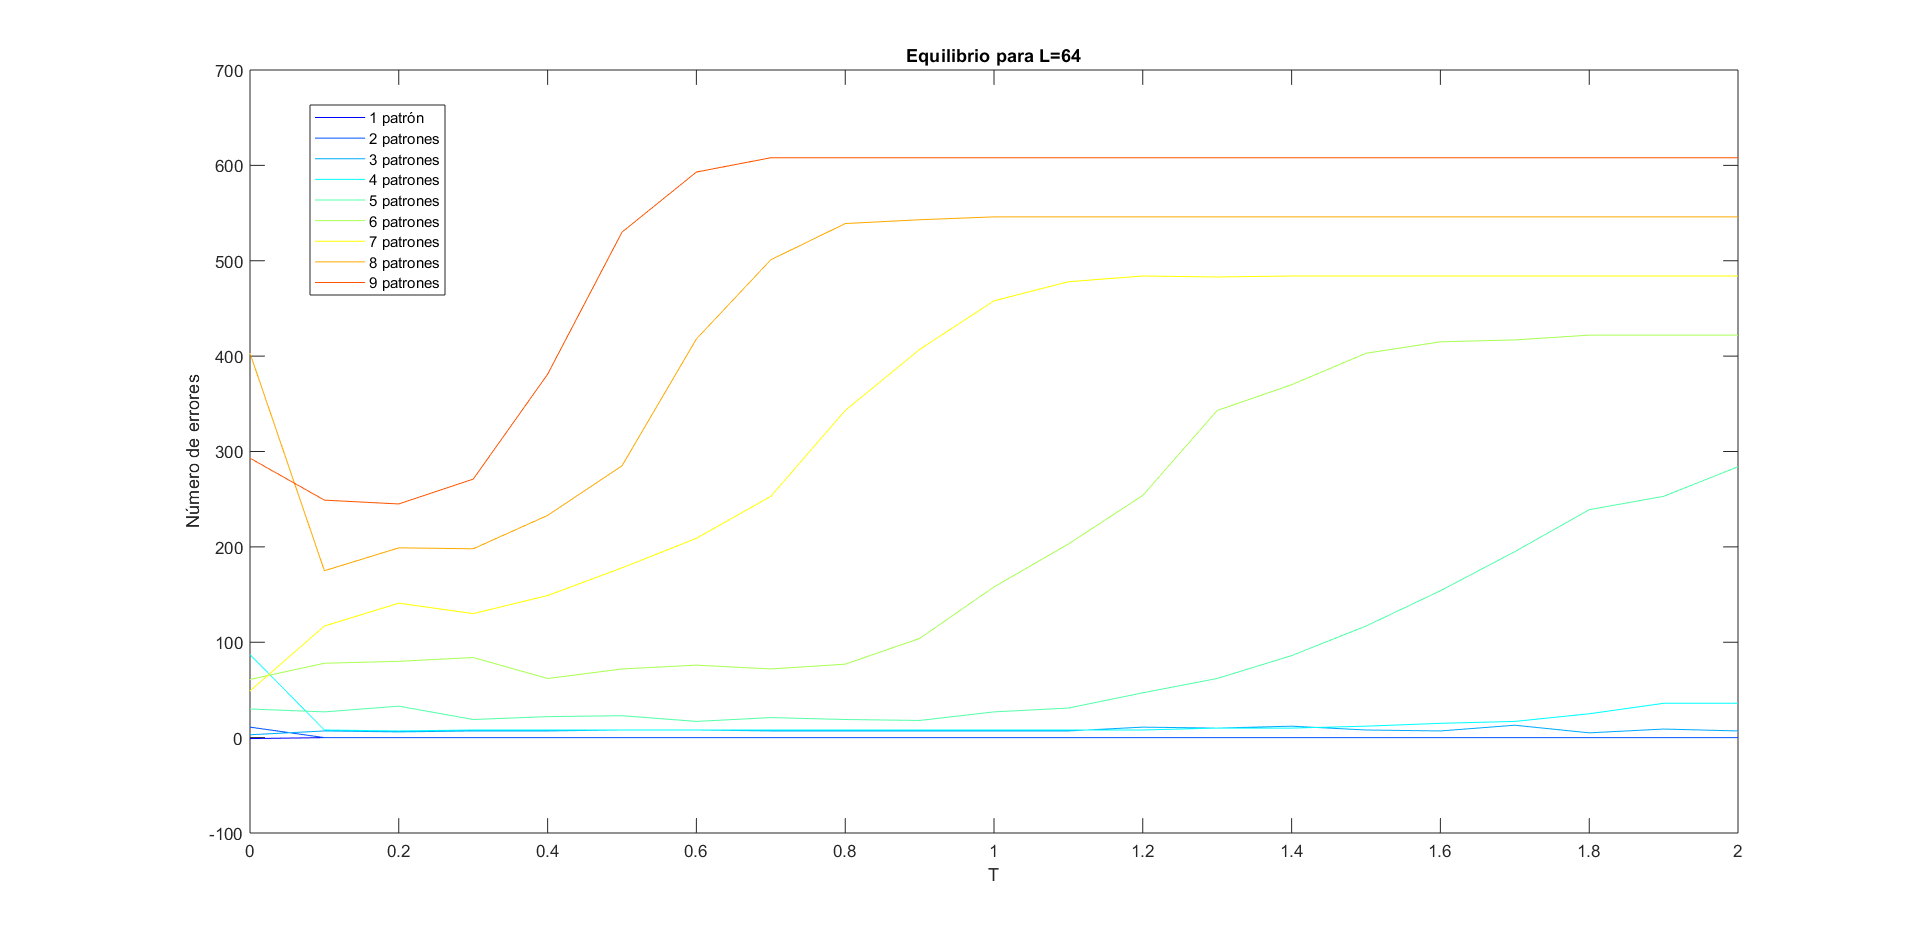
\includegraphics[scale=0.2]{dinamicaL64}
     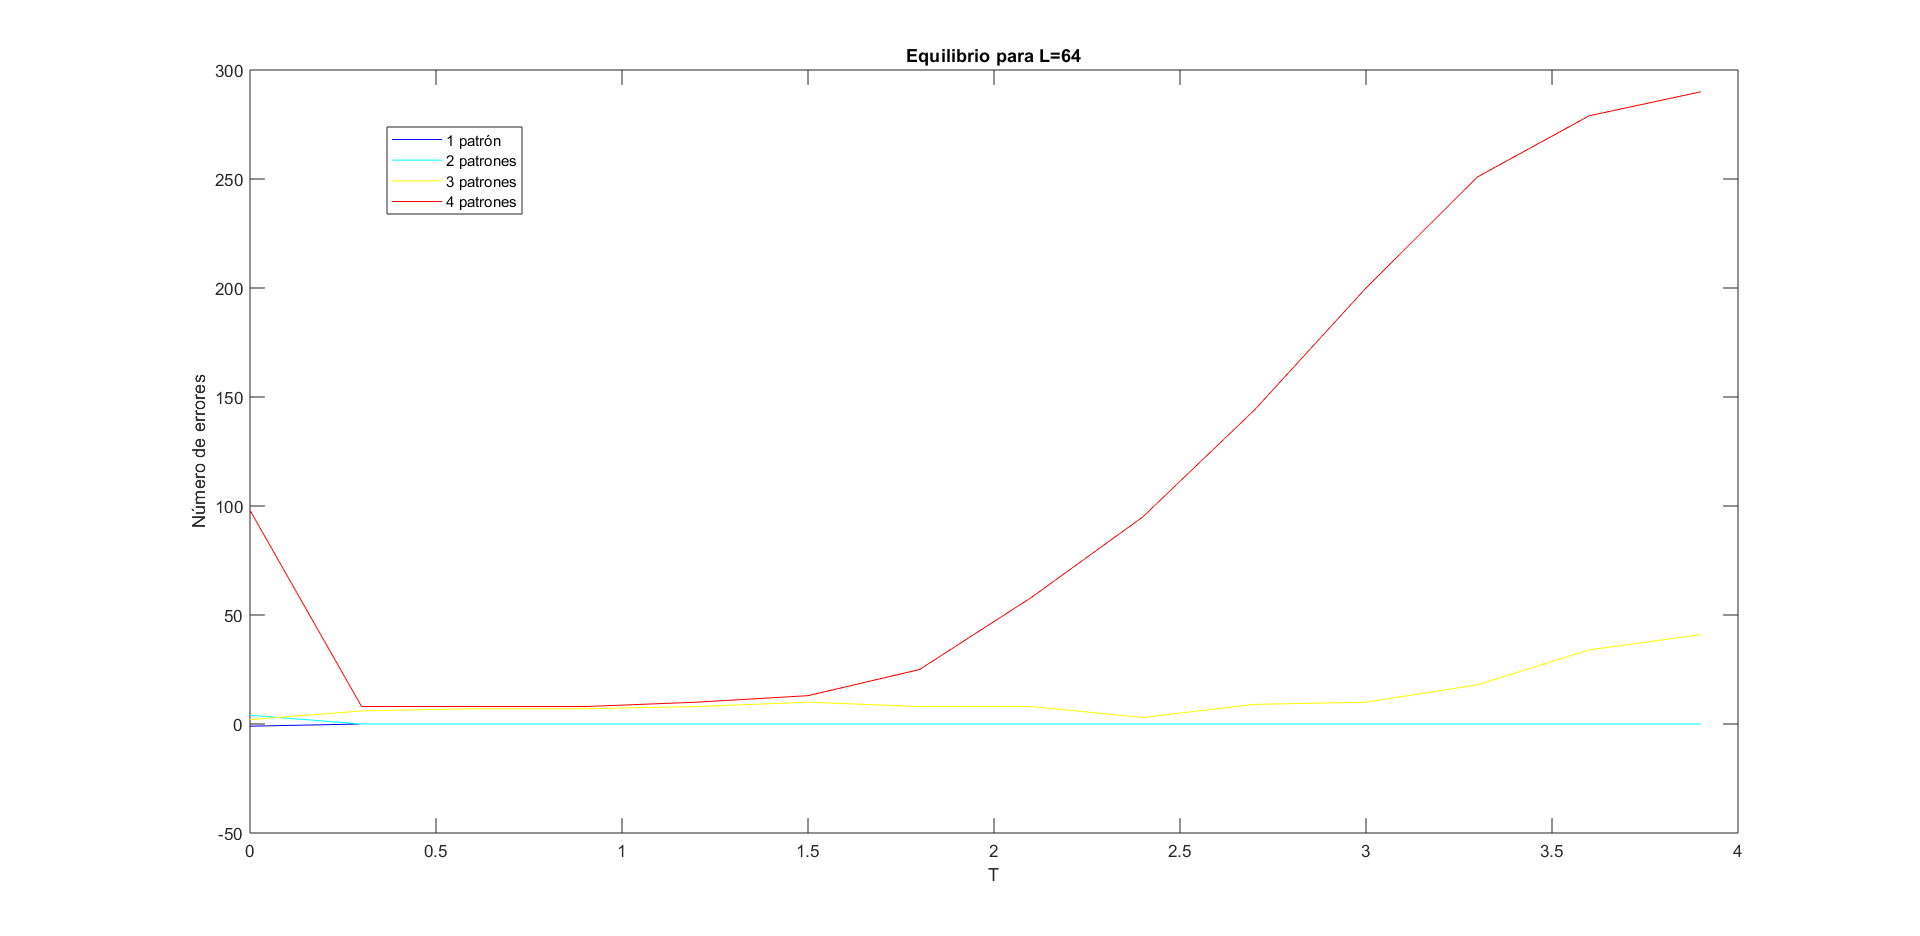
\includegraphics[scale=0.2]{dinamicaL64Talta}
 \end{center}
 Podemos ver que se reproducen los mismos comportamientos, aunque admite una cantidad mayor de patrones almacenados antes de llegar a su régimen caótico, y es capaz de tolerar la T para un número de patrones mayor que el caso L=8 , esta red no reduce a cero el número de errores, aunque sí los mantiene acotados.\\
 Para concluir esta sección, hemos visto que la evolución de la ecuación de Langevin se comportan de una manera esperada, aunque nos encontramos problemas con los estados ortogonales (lo cual nos impide evolucionar el sistema en ciertos casos como hemos visto), el sistema sí que guarda los patrones que introducimos, y evoluciona hasta estos.

	\begin{thebibliography}{9}
		\bibitem[1]{hopfield82}{J. J. Hopfield, \textit{Neural networks and physical systems with emergent collective computational abilities}, Proc. Natl. Acad. Sci. USA, \textbf{79}, 2554-2558, abril de 1982.}
		\bibitem[2]{neurodyn}{W. Gerstner, W. M. Kistler, R. Naud, L. Paninski, \textit{Neuronal Dynamics}, Cambridge University Press, 2014, \href{https://neuronaldynamics.epfl.ch/online/index.html}{https://neuronaldynamics.epfl.ch/online/index.html}.}
		\bibitem[3]{feigelman86}{M. V. Feigelman, L. B. Ioffe, \textit{The Statistical Properties of the Hopfield Model of Memory}, Europhys. Lett., \textbf{1} (4), 197-201, febrero de 1986.}
		\bibitem[4]{amit1}{D. J. Amit, H. Gutfreund, H. Sompolinsky, \textit{Spin-glass models of neural networks}, Physical Review A, \textbf{32} (2), 1007-1018, agosto de 1985.}
		\bibitem[5]{amit2}{D. J. Amit, H. Gutfreund, H. Sompolinsky, \textit{Storing Infinite Numbers of Patterns in a Spin-Glass Model of Neural Networks}, Physical Review Letters, \textbf{55} (14), 1530-1533, septiembre de 1985.}
		\bibitem[6]{neurodyn-ex}{W. Gerstner, W. M. Kistler, R. Naud, L. Paninski, \textit{Neuronal Dynamics: Python Exercises}, \href{https://neuronaldynamics-exercises.readthedocs.io/en/latest/index.html}{https://neuronaldynamics-exercises.readthedocs.io/en/latest/index.html}.}
	\end{thebibliography}
\end{document}
